% add section on what phages do in the environemnt, in general. Dont constrain to applications of the phages, talk about what they do, in the larger environemnt ecosystem, carbon turnover, 30% (depends on ecosystem) of bacterial lysis per day. (done)


% Read review from matti

% add section on thesis overview, how I created the tools and run the visualizations/analysis (done)

% In the different models (2.1), mention how phages and resources can be added to the model itself. 
% flip it around to say how you build form modelling just bacteria, maybe resources, to adding resources and phages. 
% add section 2.1.5 on a model that specifically models phages. 
% tell how the Geng model cna be made form the other 2.1.1-4 models. 

% Repression of DNA be more general, move outside and mention that you cna go to lytic or lysogenic part

% holin to lyse bacteria (done)

% do I really need fitness vlaue of the cell, and horizontal gene transfer? Maybe a bit too much, cut it down, or just rmeove it? (done, by cutting parts of it)

% CHange “good plot” to something like “this is waht typically looks like in a lab”. (done)




%%%%%%%%%%%%%%%%%%%%%%%%%%%%%%%%%%%%%%%%%
% Masters/Doctoral Thesis 
% LaTeX Template
% Version 1.43 (17/5/14)
%
% This template has been downloaded from:
% http://www.LaTeXTemplates.com
%
% Original authors:
% Steven Gunn 
% http://users.ecs.soton.ac.uk/srg/softwaretools/document/templates/
% and
% Sunil Patel
% http://www.sunilpatel.co.uk/thesis-template/
%
% License:
% CC BY-NC-SA 3.0 (http://creativecommons.org/licenses/by-nc-sa/3.0/)
%
% Note:
% Make sure to edit document variables in the Thesis.cls file
%
% Modified and Adapted by Michael Lees 2020
%%%%%%%%%%%%%%%%%%%%%%%%%%%%%%%%%%%%%%%%%

%----------------------------------------------------------------------------------------
%	PACKAGES AND OTHER DOCUMENT CONFIGURATIONS
%----------------------------------------------------------------------------------------

\documentclass[11pt, oneside, draft]{Thesis}
% \documentclass[11pt, oneside, final]{Thesis}

\graphicspath{{Images/}} 
\usepackage[square, numbers, comma, sort&compress]{natbib} % Use the natbib reference package - read up on this to edit the reference style; if you want text (e.g. Smith et al., 2012) for the in-text references (instead of numbers), remove 'numbers' 
\usepackage[ruled,vlined]{algorithm2e}
\usepackage{amsmath}
\usepackage{booktabs}
\usepackage[nameinlink]{cleveref}
\PassOptionsToPackage{hyphens}{url}
\usepackage{hyperref}
\usepackage{array}
\usepackage[svgnames]{xcolor}
\usepackage{textcomp}
\usepackage[font=small,labelfont=bf]{caption}
\usepackage{float}
\usepackage{subcaption}
\usepackage{tabularx}
% \usepackage[margin=1in]{geometry} % Adjust margins if needed
\usepackage{booktabs}    
\usepackage{listings}
\usepackage{bm}
\usepackage{aliascnt}
\usepackage{algpseudocode}
\usepackage{makecell}
\floatstyle{ruled}
\newfloat{listing}{htbp}{lop}
\floatname{listing}{Algorithm}
\newsavebox{\codebox}
\newaliascnt{eqfloat}{equation}
\newfloat{eqfloat}{h}{eqflts}
\floatname{eqfloat}{Equation}
\newcommand*{\ORGeqfloat}{}
\let\ORGeqfloat\eqfloat
\def\eqfloat{%
  \let\ORIGINALcaption\caption
  \def\caption{%
    \addtocounter{equation}{-1}%
    \ORIGINALcaption
  }
  \ORGeqfloat
}
\DeclareMathAlphabet{\mathcal}{OMS}{cmsy}{m}{n}
\SetMathAlphabet{\mathcal}{bold}{OMS}{cmsy}{b}{n}

% styling used for code color in appendix D
\definecolor{codegreen}{rgb}{0,0.6,0}
\definecolor{codegray}{rgb}{0.5,0.5,0.5}
\definecolor{codepurple}{rgb}{0.58,0,0.82}
\definecolor{backcolour}{rgb}{0.95,0.95,0.92}
\lstdefinestyle{codestyle}{
    backgroundcolor=\color{backcolour}, 
    commentstyle=\color{codegreen}, 
    keywordstyle=\color{magenta}, 
    numberstyle=\tiny\color{codegray}, 
    stringstyle=\color{codepurple}, 
    basicstyle=\ttfamily\footnotesize, 
    breakatwhitespace=false, 
    breaklines=true, 
    captionpos=b, 
    language=Python, 
    keepspaces=true, 
    numbers=left, 
    numbersep=10pt, 
    showtabs=false, 
    tabsize=2 
}

% For better horizontal rules
\DeclareMathOperator*{\argmin}{arg\,min} 
\DeclareMathOperator*{\argmax}{arg\,max}
\DeclareCaptionType{equ}[][]
\hypersetup{colorlinks=true, filecolor=magenta, urlcolor=cyan, linkcolor=blue} % Colors hyperlinks in blue - change to black if annoying
\urlstyle{same}
\title{\ttitle} % Defines the thesis title - don't touch this
\begin{document}
\frontmatter 
\setstretch{1.3} 

\fancyhead{} 
\rhead{\thepage} 
\lhead{}

\pagestyle{fancy} % Finally, use the "fancy" page style to implement the FancyHdr headers

\newcommand{\HRule}{\rule{\linewidth}{0.5mm}} 

\hypersetup{pdftitle={\ttitle}}
\hypersetup{pdfsubject=\subjectname}
\hypersetup{pdfauthor=\authornames}
\hypersetup{pdfkeywords=\keywordnames}

%----------------------------------------------------------------------------------------
%	TITLE PAGE
%----------------------------------------------------------------------------------------

\begin{titlepage}
\begin{center}

\textsc{\LARGE \univname}\\[1.5cm] % University name
\textsc{\Large Masters Thesis}\\[0.5cm] % Thesis type

\HRule \\[0.4cm] % Horizontal line
{\huge \bfseries \ttitle}\\[0.4cm] % Thesis title
\HRule \\[1.5cm] % Horizontal line
 
\begin{minipage}{0.4\textwidth}
\begin{flushleft} \large
\emph{Author:}\\
\authornames % Author name - remove the \href bracket to remove the link
\end{flushleft}
\end{minipage}
\begin{minipage}{0.4\textwidth}
\begin{flushright} \large
\emph{Examiner:} \\
{\exname}\\
\emph{Supervisor:} \\
{\supname}\\
\emph{Assessor:} \\
{\assessorname}
\end{flushright}
\end{minipage}\\[1cm]
 
\large \textit{A thesis submitted in partial fulfillment of the requirements\\ for the degree of \degreename}\\[0.3cm] % University requirement text
\textit{in the}\\[0.4cm]
\groupname\\\deptname\\[1cm] % Research group name and department name
 
{\large \todayy}\\[2cm] % Date
\includegraphics[width=0.6\textwidth]{clslogo.png} % Include Computational Science Logo
 
\vfill
\end{center}

\end{titlepage}

%----------------------------------------------------------------------------------------
%	DECLARATION PAGE
%	Your institution may give you a different text to place here
%----------------------------------------------------------------------------------------

\Declaration{

\addtocontents{toc}{\vspace{1em}} % Add a gap in the Contents, for aesthetics

I, \authornames, declare that this thesis, entitled `\ttitle' and the work presented in it are my own. I confirm that:

\begin{itemize} 
\item[\tiny{$\blacksquare$}] This work was done wholly or mainly while in candidature for a research degree at the University of Amsterdam.
\item[\tiny{$\blacksquare$}] Where any part of this thesis has previously been submitted for a degree or any other qualification at this University or any other institution, this has been clearly stated.
\item[\tiny{$\blacksquare$}] Where I have consulted the published work of others, this is always clearly attributed.
\item[\tiny{$\blacksquare$}] Where I have quoted from the work of others, the source is always given. With the exception of such quotations, this thesis is entirely my own work.
\item[\tiny{$\blacksquare$}] I have acknowledged all main sources of help.
\item[\tiny{$\blacksquare$}] Where the thesis is based on work done by myself jointly with others, I have made clear exactly what was done by others and what I have contributed myself.\\
\end{itemize}


Signed: \\\\\includegraphics[width=3cm]{Images/signature.pdf} \\
%\rule[1em]{25em}{0.5pt} % This prints a line for the signature
 
Date: \today\\
%\rule[1em]{25em}{0.5pt} % This prints a line to write the date
}

\clearpage % Start a new page

%----------------------------------------------------------------------------------------
%	QUOTATION PAGE
%----------------------------------------------------------------------------------------

\pagestyle{empty}
\null\vfill 
\textit{``All models are wrong, but some are useful``}
\begin{flushright}
    George E. P. Box
\end{flushright}
\vfill\vfill\vfill\vfill\vfill\vfill\null 
\clearpage 

%----------------------------------------------------------------------------------------
%	ABSTRACT PAGE
%----------------------------------------------------------------------------------------
\addtotoc{Abstract} 
\abstract{\addtocontents{toc}{\vspace{1em}} 
    In any given microbial ecosystem, there can be hundreds of different phages and bacteria interacting with one another in a complex system. 
    These individual interactions have a significant impact on the bacterial community and the overall ecosystem, with important ecological consequences. 
They force bacteria to mutate and evolve, changing the community fitness level. 
    Phages can control bacterial populations, ensuring that dangerous bacteria do not over-reproduce and harm the ecosystem. 
    Phages control bacterial population dynamics using the “kill-the-winner” dynamic, preventing any one species from dominating.
    Upon lysis, bacteria release resources into the environment that other bacteria and plants can use. 

    There is a need to mathematically model complex systems, but current models typically only model 1 or 2 phages and bacteria. 
    It is, however, straightforward to extend the model to multiple species. 
    Mathematically modeling large bacterial communities is important because running lab experiments takes time and is costly. 
    These simulations can guide future lab work, for example, in combating antibiotic-resistant bacteria. 

    I created a program consisting of three parts that can model complex communities of $p$ phages, $b$ bacteria, and $r$ resources. 
    The first part uses a GUI tool to create and edit the interactions between the phages, bacteria, and resources using a graph network. 
    The nodes and edges hold the interaction and environmental parameter values. 
    The second part, the simulation framework itself, models and calculates the phage, bacteria, and resource population levels with the user-provided network and ODE model. 
    The third part allows the user to interact with the simulation framework with a custom-built dashboard. 
    The user can, for example, change the parameter values from the dashboard and immediately see how the change affects the simulation. 
    There are five pre-built plots that the user can interact with. 
    It is possible to download the simulation results so that the user can create custom analyses and plots. 

    I apply this process to the Golding model from \citet{gengUsingBacterialPopulation2024}. 
    I qualitatively analyze the model's behavior and use a SOBOL analysis to quantitatively assign a value to the model's variance in output from the model's input. 
    In addition, understanding the different regimes of restriction in phages, as well as the factors that drive reaction rates and determine the rate-limiting steps, is crucial.
    By varying the initial uninfected bacteria population, the model can interpolate between two limiting scenarios, adsorption and latency limited. 
    It is important to determine whether a phage population will proliferate in a laboratory context under constant washout to prevent the phage population from accidentally being wiped out. 
    I run an analysis to see if phages will proliferate or die out depending on the initial condition. 
    Finally, I perform and analyze a co-existence analysis on a large 20-phage, 20-bacteria, and 10-resource community to determine whether phages and bacteria can coexist under various conditions. 
    I find that in large communities, phages and bacteria can coexist. 
    If a debris term is introduced, the bacteria's survivability rate increases.

% Include your abstract here 
% Abstracts must include sufficient information for reviewers to judge the nature and significance
% of the topic, the adequacy of the investigative strategy, the nature of the results, and the
% conclusions. The abstract should summarize the substantive results of the work and not merely
% list topics to be discussed. 
% Length 200-400 words.
}
\clearpage 

%----------------------------------------------------------------------------------------
%	ACKNOWLEDGEMENTS
%----------------------------------------------------------------------------------------

\setstretch{1.3} 
\acknowledgements{
    \addtocontents{toc}{\vspace{1em}} 
    I would like to thank my parents for loving me despite some of my faults, and for supporting me through my Bachelor and Master studies even if they don't exactly know what I am studying. Without them, I wouldn't know where my life would be right now, and I certainly would be a different person if it were not for them. 

    Thank you to Dr. Matti Gralka for the weekly meetings and teaching me everything about phages and bacteria. 
    Every meeting was always insightful, productive, and informative. 
    I will forever be amazed at how he can remember which paper talks about which topic, and how he always had a paper for every topic. 

    Thank you to Sofia Blaszczyk for finding the Master thesis opening and suggesting that I email Dr. Gralka for an introductory meeting. 
    She acted as my \href{https://www.wikiwand.com/en/articles/Rubber_duck_debugging}{rubber duck programming buddy}, and watched my cringe screen recordings that I sent her at 2am showcasing various demos of my project. 
    If she wouldn't have found this opening, I wouldn't know what I would be doing as my thesis. 

    If I hadn't followed Dr. Rik Kaasschieter's and Dr. Martijn Anthonissen's courses “Introduction Computational Sciences“ and “Numerical Linear Algebra“ in my Bachelors, I would not have been interested in Computational Sciences. 
    I would not have found the MSc Computational Sciences program, as Computational Sciences fits my interests and skill sets better than any other program I could have taken. 
    For Rik and Martijn have forever altered my career trajectory. 

    Thank you to Sarah Flickinger for showing me the research that she has been doing in the lab. 
    She allowed me to really connect my research and models to real life, reminding me that what I am doing has real life use cases than just a purely theoretical or programming challenge. 

    And finally, thank you to all of my friends for keeping me sane and helping me through both of my programs. 
}
\clearpage 

%----------------------------------------------------------------------------------------
%	LIST OF CONTENTS/FIGURES/TABLES PAGES
%----------------------------------------------------------------------------------------

\pagestyle{fancy} 
\lhead{\emph{Contents}} 
\tableofcontents 
\lhead{}

\lhead{\emph{List of Figures}} 
\listoffigures 
\lhead{}

\lhead{\emph{List of Tables}}
\listoftables
\lhead{}

% \lhead{\emph{List of Algorithms}}
% \addtotoc{List of Algorithms}
% \listofalgorithms
% \lhead{}

%----------------------------------------------------------------------------------------
%	ABBREVIATIONS
%----------------------------------------------------------------------------------------

\clearpage 
\setstretch{1.5}
\lhead{\emph{Abbreviations}}
\listofsymbols{ll}
{
    % \textbf{ABM} & \textbf{A}gent \textbf{B}ased \textbf{M}odelling \\ 
    % \textbf{ARD} & \textbf{A}rms \textbf{R}ace \textbf{D}ynamic \\ 
    % \textbf{BVP} & \textbf{B}oundary \textbf{V}alue \textbf{P}roblem \\ 
    % \textbf{CBASS} & \textbf{C}yclic oligonucleotide-\textbf{B}ased \textbf{A}ntiphage \textbf{S}ignalling \textbf{S}ystems\\
    % \textbf{CRISPR} & \textbf{C}lustered \textbf{R}egularly \textbf{I}nterspaced \textbf{S}hort \textbf{P}alindromic \textbf{R}epeats \\
    \textbf{DDE} & \textbf{D}elay \textbf{D}ifferential \textbf{E}quation \\ 
    \textbf{DNA} & \textbf{D}eoxyribo\textbf{N}ucleic \textbf{A}cid \\
    % \textbf{FSD} & \textbf{F}luctuating \textbf{S}election \textbf{D}ynamics \\ 
    \textbf{GUI} & \textbf{G}raphical \textbf{U}ser \textbf{I}nterface \\ 
    \textbf{IC} & \textbf{I}nitial \textbf{C}ondition \\
    \textbf{IVA} & \textbf{I}nitial \textbf{V}alue \textbf{A}nalysis \\ 
    \textbf{OD} & \textbf{O}ptical \textbf{D}ensity \\ 
    \textbf{ODE} & \textbf{O}rdinary \textbf{D}ifferential \textbf{E}quation \\
    \textbf{PA} & \textbf{P}arameter \textbf{A}nalysis \\
    \textbf{PDE} & \textbf{P}artial \textbf{D}ifferential \textbf{E}quation \\ 
    \textbf{RNA} & \textbf{R}ibo\textbf{N}ucleic \textbf{A}cid\\
    % \textbf{SIE} & \textbf{S}uper\textbf{I}nfection \textbf{E}xclusion \\
    % \textbf{SNP} & \textbf{S}ingle \textbf{N}ucleotide \textbf{P}olymorphism \\
    \textbf{ST} & \textbf{S}erial \textbf{T}ransfer\\ 
    % \textbf{TAB} & \textbf{T}ail \textbf{A}ssembly \textbf{B}locker \\
    \textbf{UA} & \textbf{U}ltimate \textbf{A}nalysis \\
    \textbf{UvA} & \textbf{U}niversitiet \textbf{v}an \textbf{A}msterdam\\
}
\lhead{}

%----------------------------------------------------------------------------------------
%	PHYSICAL CONSTANTS/OTHER DEFINITIONS
%----------------------------------------------------------------------------------------

\clearpage 

%\lhead{\emph{Physical Constants}} % Set the left side page header to "Physical Constants"

%\listofconstants{lrcl} % Include a list of Physical Constants (a four column table)
%{
%Speed of Light & $c$ & $=$ & $2.997\ 924\ 58\times10^{8}\ \mbox{ms}^{-\mbox{s}}$ (exact)\\
%% Constant Name & Symbol & = & Constant Value (with units) \\
%}

%----------------------------------------------------------------------------------------
%	SYMBOLS
%----------------------------------------------------------------------------------------

\clearpage

% \lhead{\emph{Symbols}} 

% A table of Symbols and Parameter Values can be viewed in \Cref{AppendixA} and \Cref{AppendixE}. 
% \listofnomenclature{lll} % Include a list of Symbols (a three column table)
% {
% $a$ & distance & m \\
% $P$ & power & W (Js$^{-1}$) \\
% % Symbol & Name & Unit \\

% & & \\ % Gap to separate the Roman symbols from the Greek

% $\omega$ & angular frequency & rads$^{-1}$ \\
% % Symbol & Name & Unit \\
% }

%----------------------------------------------------------------------------------------
%	DEDICATION
%----------------------------------------------------------------------------------------

\setstretch{1.3} 
\pagestyle{empty} 
\addtocontents{toc}{\vspace{2em}} 

%----------------------------------------------------------------------------------------
%	THESIS CONTENT - CHAPTERS
%----------------------------------------------------------------------------------------

\mainmatter
\pagestyle{fancy}

%This structure provides a bare bones essentials of the thesis and some indicative length
%This structure may not fit your thesis perfectly, but be sure to include these components somehow.
%It is possible to split the chapters up (E.g., 2 methods chapter, Experiment and Results as two, etc.)

% The typical length may be between 43 - 64 pages. Do not worry if you go slightly larger or smaller than this. 
% But a thesis of 20 pages, or 100 pages may suggest you've been to brief or too verbose.
%NOTE - there is not strict limit/minimum.

\lhead{\emph{Introduction}}
\chapter{Introduction}
\label{Introduction}

Phages are small viruses on the order of 27-190nm that infect and lyse (kill) specific bacteria, acting as nature's natural anti-microbial defense. 
Researchers are attempting to determine how phages can be used in various medical and industrial applications to control bacterial growth. 
However, researchers need to know how the interactions between phages and bacteria work in order to implement a robust method to control bacterial growth. \newline 

\section{Biological Background}
Phages are small viruses on the order of 27-190nm that infect and lyse (kill) specific bacteria.
The phage cycle process starts with a phage coming into contact with a bacterium.
Once it has identified an injection site, the phage can inject a strain of DNA into the bacteria.
The DNA strand has two options: it can either merge into the bacterial DNA, allowing the phage's DNA strand to replicate alongside the bacteria as they reproduce.
This process defines the Lysogenic cycle.
After a set amount of time, the DNA of the phage can unmerge and hijack the DNA replicating mechanism, creating multiple copies of itself, using the transcription, translation, and replication process to create multiple copies of itself.
The phages begin to self-assemble inside the bacteria until the bacteria is full of phages and explodes, the lysis stage, releasing the phages into the environment, ready to repeat the process again. 

This process can be visualized in \Cref{fig:phage_life_cycle} \cite{campbellFutureBacteriophageBiology2003}.
\begin{figure}
    \centering
    \includegraphics[width=0.5\linewidth]{Figures/phage_life_cycle.png}
    \caption{Life cycle of a phage, inside and outside a bacteria cell. Significant steps in the life cycle of a phage include the infection stage, integration, replication, and lysing process. Figure sourced from \citet{campbellFutureBacteriophageBiology2003}. }
    \label{fig:phage_life_cycle}
\end{figure}

\section{Phage Cocktail and Human Health}
There is particular interest in phage applications in human and animal health, called phage cocktail therapy, due to phage cocktails not exhibiting side effects.
Phage cocktails are a medicine that sick patients with bacterial diseases, such as \textit{Escherichia coli} can use. 
A patient can swallow a pill filled with a range of different phages that target \textit{E. coli}.
The phages will target the specific \textit{E. coli} bacteria, but it will not affect the other bacteria found in the gut of the human body and will not have any side effects on the body. 
There are about 100 trillion microbes across 5,000 different types of bacteria strains in the human gut. 
Antibiotics disrupt the intricate ecosystem of the gut microbiome, acting as a scorched-earth mechanism. 
Phages on the other hand specifically target a specific bacterial strain, acting as a sniper, with minimal to no effects to other bacterial strains, while antibiotics act as a bomb. 
A challenge that antibiotics face is that antibiotics create antibiotic resistant bacteria, making the antibiotic less effective in the future \cite{odonkorBacteriaResistanceAntibiotics2011, volkovaEffectsEarlylifePenicillin2021}. 
There is however hope that phage resistant bacteria become more susceptible to antibiotics due to changes in the cell structure \cite{laurePhageResistancemediatedTradeoffs2022, zhaoPhagedrivenCoevolutionReveals2024}. 
\nameref{sec:AppendixB:phage_therapy_and_antibiotics} in \nameref{AppendixB} goes more in depth on how phages can be used in a healthcare setting. 

\section{Industrial Usage}
Phages have many uses in an industrial setting. 
Similarly, phage therapies can be used as a preventative method, by preventing the spread of common bacteria in livestock by dosing the animal feed with the phage pills. 
Farmers often raise livestock in tight spaces with a lack of sanitation facilities, increasing the risk of a disease spreading. \newline 
Phages can be used to control the growth of bacteria like \textit{Salmonella} while producing food in a factory \cite{sofferBacteriophagesSafelyReduce2016, kowalskaFreshVegetablesFruit2023}. 
\nameref{sec:AppendixB:controlling_foodborne_bacteria} in \nameref{AppendixB} goes into more detail about using phages to control foodborne bacteria. 

\section{The Environment}
In an ecosystem like the ocean, the gut, or in soil, there are thousands of different microbes all interacting with one another or the surrounding environment.
The interactions are complex, with many factors affecting the growth of bacteria, fungi, phages, plants, animals, and more. 
Often, the interactions between agents in the environment are synergistic. 
When an animal dies, bacteria start to digest and decompose the animal into simpler chemicals like carbon and nitrogen that plants can use to grow, which is then eaten by other animals. 
Finally, phages can potentially be used to control \textit{Cyanobacteria} (blue-green algae) blooms in the environment and affect other agents such as plankton in the environment \cite{colomaFrequencyVirusresistantHosts2019}. 
\textit{Cyanobacteria} cause damage to aquatic life by consuming nutrients and oxygen, starving aquatic life. \textit{Cyanobacteria} can also affect human health by infecting drinking water. 
Having the ability to control \textit{Cyanobacteria} growth can save nature and protect human health. 
With this, there is hope that water quality can be engineered without using harsh chemical processes what would otherwise pose environmental and health hazards \cite{tuckerIdentificationCyanophageMaLBP2005}. \newline
More information about controlling \textit{Cyanobacteria} can be read in \nameref{sec:AppendixB:environmental_protection}. 

External factors, such as flooding, droughts, chemical spills, or introduction of new agents have a massive impact on the ecosystem. 
These events can add or remove resources from the system, change environmental parameters such as the surrounding temperature, introduce competition, or create an imbalance in the population by killing agents. 
These effects have a larger effect on the ecosystem and food chain as a whole as bacteria are one of the fundamental foudnations for nutrient recycling. 

\section{Modelling Phages in a Complex Community}
Not much is known about phages in large and complex communities between other phages, bacteria, resources, and the environment. 
There have been previous attempts to model the complex dynamics of the populations between phages, bacteria, and resources, with the environment using Ordinary Differential Equations (ODE) and Delay Differential Equations (DDE).
Not every interaction in the complex community can be identified, and if an interaction has been identified, the associated parameter values are unknown and need to be experimentally derived. 
Collecting interaction parameter values is an expensive and laborious task, as the data has to experimentally collected. 

There are two main ways to model phage-bacteria dynamics: spatially and non-spatially.
In a spatial model phages and bacteria can move through space and interact with their neighbors. 
Partial differential equations (PDE) and cellular agent-based models (ABM) have been used to model spatial interactions.
Spatial models require special considerations, such as proximity to other agents.
This creates areas of interaction and interest where agents are located, and areas of no interactions where there are no interactions.
Spatial models lead to more computationally complex models, but result in more interesting results. 

Whereas in non-spatial models such as ODEs and DDEs, the bacteria and phages are assumed to be in a well-mixed solution and no distinctions are made in regard to neighbors or distances to other agents. 
Interactions are simplified to a probabilistic approach, where a percentage $p$ of agents interact with one another at time step $t$.
Non non-spatial models are easier to develop, understand, and are more effective in modeling large populations, at the cost of losing spatial information. 

For this thesis, the focus will be modelling resource, phage, and bacteria interactions using an ODE model. 
A phage-bacteria-resource system is described as an $p\times b \times r$ system, meaning $p$ phages, $b$ bacteria, 
Current modelling methods have mainly stayed with $1\times 1 \times 1$ models, meaning 1 phage, 1 bacteria, and 1 resource. 
This thesis aims to develop a simulation framework that can model any $p\times b \times r$ system, where each agent can contain states (called hidden agents) that they can move to and from. 
\newline 

\section{Thesis Project}
The project is divided into three logical parts, with an optional fourth part.
The first section is to create the network interaction. 
Here the user of the software can define the number of resources, phages, and bacteria, who interacts with who, and the strength and type of interactions. See \nameref{sec:network_creation_tool} for further information. \newline
In \nameref{sec:simulation_framework}, the user uploads the network model and parameters and as output receives the time data and population data as an array. \newline
\nameref{sec:visualization_framework} allows the user to interact with \nameref{sec:network_creation_tool} and \nameref{sec:simulation_framework} with a dashboard. 
The user can graphically edit the attribute values of the edges and nodes of the network, and the user can run more advanced visualizations, for example by changing a parameter value and seeing how that affects the population count. 
There are a few plots included out of the box that the user can test. 
The plots offered in part 3 offer interactivity like hiding and showing lines and dots, zooming in and out, and hovering over the lines and dots to show more details of the data. 
\newline
Finally, the user can optionally run multiple simulations and download the data to their disk to create their own custom visualizations using \nameref{sec:custom_visualization_and_framework}. 
The visualizations created in \nameref{sec:visualization_framework} can theoretically be recreated in \nameref{sec:custom_visualization_and_framework}. 
The user can choose the same parameter values used for a specific plot in \nameref{sec:visualization_framework}, run the simulation (under the \nameref{sec:ultimate_analysis} section), download the data, and reimplement the graphs.  %Set out your thesis and state your research question (5-8 pages)
\newpage

\lhead{\emph{Literature Review}}
\chapter{Literature review}
\label{LR}

\section{Methods of Modelling Phages and Bacteria}
There are numerous ways to model the interactions between phages and bacteria.
Populations of phages, bacteria, and resources are typically modeled using Ordinary Differential Equations (ODEs) or Delay Differential Equations (DDE). 
DDEs are similar to ODEs, but DDEs incorporate time delays to account for processes that depend not only on the current state but also on past states, such as latency periods in phage infection or delayed bacterial responses to environmental changes.

One way to introduce a delay in an ODE model is to force populations to go through stages, causing a delay in other events. 
For example, in the paper \citet{gengUsingBacterialPopulation2024}, infected bacteria go through $M$ stages of infection, before lysing. 
By decreasing $\tau$ (the latent period) in the model proposed by \citet{gengUsingBacterialPopulation2024}, the throughput of bacteria going from stage $i$ to stage $i+1$ of infection increases, thus seeing a larger rise in phage population. 
All simulations and analyses in this report will use the Golding model, see \Cref{sec:golding_model}. 

Each type of model has its pros and cons.
With the molecular level model, the model is more complex and needs significantly more startup time, simulation time, and is much more complex.
However, more information can be gained from the simulations and can guide research in creating phages for a certain type of bacteria.
The ODE method is simpler to understand and easier to set up, but it can only capture large population dynamics.
Certain assumptions about the community interactions also have to be made, such as the constant washout of the bacteria. 
Each model can be further developed, for example by adding temperature and pH dependence, bacteria releasing nutrients, or if the bacteria concentration is above a certain threshold, the infection rate is lowered to model phages struggling to diffuse through a biofilm. 

\subsection{Generalized Lotka-Volterra Model}
The Lotka-Volterra model, a first-order non-linear differential model, captures the dynamics between predators and prey.
Any population can be modelled as such:
\[ 
    \frac{d{B}_i}{dt} = {B}_i \left(\left(r_i + \sum_{j}^{N} \alpha_{ij}{B}_j \right) - m_i\right)
\]
where $r_i$ is reproduction rate, $\alpha_{ij}$ is the devour rate of $B_i$ on $B_j$. If $\alpha_{ij}$ is negative, then $B_i$ has a negative effect on $B_j$, otherwise $B_i$ has a positive effect on $B_j$. $m_i$ is the removal rate of $B_i$. 
The interactions can be seen in \Cref{fig:lotka_volterra_model}. 

It is possible to add phages into the system by 
 
\subsection{Generalized Consumer-Resource Model}
The generalized Consumer-Resource Model models the growth of a population and resource dynamics between a population of bacteria ${B}_i$ and a resource ${R}_i$. 
\begin{align}
    \frac{d{B}_i}{dt} &= r_i{B}_i \left(\sum_{\alpha} \Delta w_{i \alpha}C_{i \alpha}R_{\alpha}\right) - m_i {B}_i \label{eq:generalized_consumer_resource_model_1}\\
    \frac{dR_{\beta}}{dt} &= -\sum_i C_{i\beta}R_{\beta}{B_i} + \sum_{\alpha, i}D_{\beta\alpha}^{i}C_{i\alpha}R_{\beta}{B}_i \label{eq:generalized_consumer_resource_model_2}\\
    \Delta w_{i\alpha} &= \sum_{\beta}D_{\beta \alpha}^{i}w_{\beta} \nonumber
\end{align}
\Cref{eq:generalized_consumer_resource_model_1} describes the growth of population $B_i$ and \Cref{eq:generalized_consumer_resource_model_2} describes the resource dynamics and metabolism of resource $R_\beta$. 
Resource $R_\alpha$ can become resource $R_\beta$ at rate $R_{\beta \alpha}^{i}$. 
Bacteria $B_i$ reproduces at rate $r_i$ dependent on the concentration of resources $\sum_\alpha C_{i\alpha}$. 
Bacteria die out at rate $m_i$. 
For a visual, see \Cref{fig:consumer_resource_model}

\subsection{Agent-Based Models}
In contrast to Lotka-Volterra and consumer-resource models, ABMs model individual agents and their interactions with other agents and the environment through space and time.
Agents interact with other agents in the vicinity according to some preset rules. 
Non-agent-based entities, such as resources, can diffuse through the environment and are typically modeled using partial differential equations (PDEs) to solve boundary value problems. 
Agents themselves may move between locations with a probability $p$, which can depend on environmental factors or stochastic processes.  
ABMs are used when there is a need to simulate individual entities. 

\begin{align} 
    \label{eq:resource_diffusion}
    \frac{\delta R_\alpha(\left(x, y\right), t)}{\delta t} = \nabla \left[D \left( R_\alpha, \left(x, y\right) \right) \nabla R_\alpha \left(\left(x, y\right), t \right) \right]
\end{align}
\Cref{eq:resource_diffusion} describes the diffusion of resource $R_\alpha$ through space, dependent on the resource concentration $R_\alpha$ at location $(x, y)$. 
The rules for cellular agents follow \Cref{eq:agent_rules}. 
\begin{align} 
    \label{eq:agent_rules}
    \frac{di}{dt} = r_i \left( \sum_\alpha \Delta w_{i\alpha}C_{i\alpha}R_\alpha\right)
\end{align}, 
where $i$ is a bacterial agent. 
\begin{align} 
    \label{eq:agent_consumption_and_conversion}
    \frac{dR_\beta}{dt} &= \sum_i C_{i\beta}R_\beta I + \sum_{\alpha, i}D_{\beta \alpha}^{i} C_{i \alpha} R_\alpha i
\end{align}
\Cref{fig:agent_based_model} shows how the agents interact with other agents in their cell. 

\begin{figure}[h!]
    \centering
    \begin{subfigure}{0.49\linewidth}
        \centering
        \captionsetup{width=1\linewidth}
        \includegraphics[width=\linewidth]{Figures/lotka_volterra_model.png}
        \caption{
            Lotka-Volterra model.
        }
        \label{fig:lotka_volterra_model}
    \end{subfigure}
    \hfill
    \begin{subfigure}{0.49\linewidth}
        \centering
        \captionsetup{width=1\linewidth}
        \includegraphics[width=\linewidth]{Figures/consumer_resource_model.png}
        \caption{
            Consumer Resource model.
        }
        \label{fig:consumer_resource_model}
    \end{subfigure}
    \hfill
    \begin{subfigure}{0.49\linewidth}
        \centering
        \captionsetup{width=1\linewidth}
        \includegraphics[width=\linewidth]{Figures/trait_based_model.png}
        \caption{
            Trait Based model. 
        }
        \label{fig:trait_based_model}
    \end{subfigure}
    \hfill
    \begin{subfigure}{0.49\linewidth}
        \centering
        \captionsetup{width=1\linewidth}
        \includegraphics[width=\linewidth]{Figures/agent_based_model.png}
        \caption{
            Agent Based model. 
        }
        \label{fig:agent_based_model}
    \end{subfigure}
    \caption{Different models and how the bacterial entities interact with itself, one another, resources and the environment. All figures sourced from \citet{vandenbergEcologicalModellingApproaches2022}}. 
\end{figure}


\section{Phage Biology}
\subsection{What Are Phages?}
Phages are small bundles of proteins that contain viral DNA. 
Phages are made up of multiple parts built like LEGO to complete the task of infecting a bacterium. 
\Cref{fig:figures:phage_diagram} shows the body parts of a phage. 
The aim of the phage is to find a suitable bacterial host and infect the host with viral DNA. 
The DNA alters the host's metabolic pathways to its benefit and hijacks the cellular replication process to create new copies of the phage. 
Eventually, the cell lyses, releasing the newly created phages into the environment to infect more bacteria. 
\begin{figure}[h!]
    \centering
    \begin{subfigure}{0.25\linewidth}
        \centering
        \captionsetup{width=1\linewidth}
        \includegraphics[width=\linewidth]{Figures/phage_diagram.png}
        \caption{
            Phage body structure. 
            % (https://www.newyorker.com/tech/annals-of-technology/phage-killer-viral-dark-matter). 
        }
        \label{fig:figures:phage_diagram}
    \end{subfigure}
    \hfill
    \begin{subfigure}{0.3\linewidth}
        \centering
        \captionsetup{width=1\linewidth}
        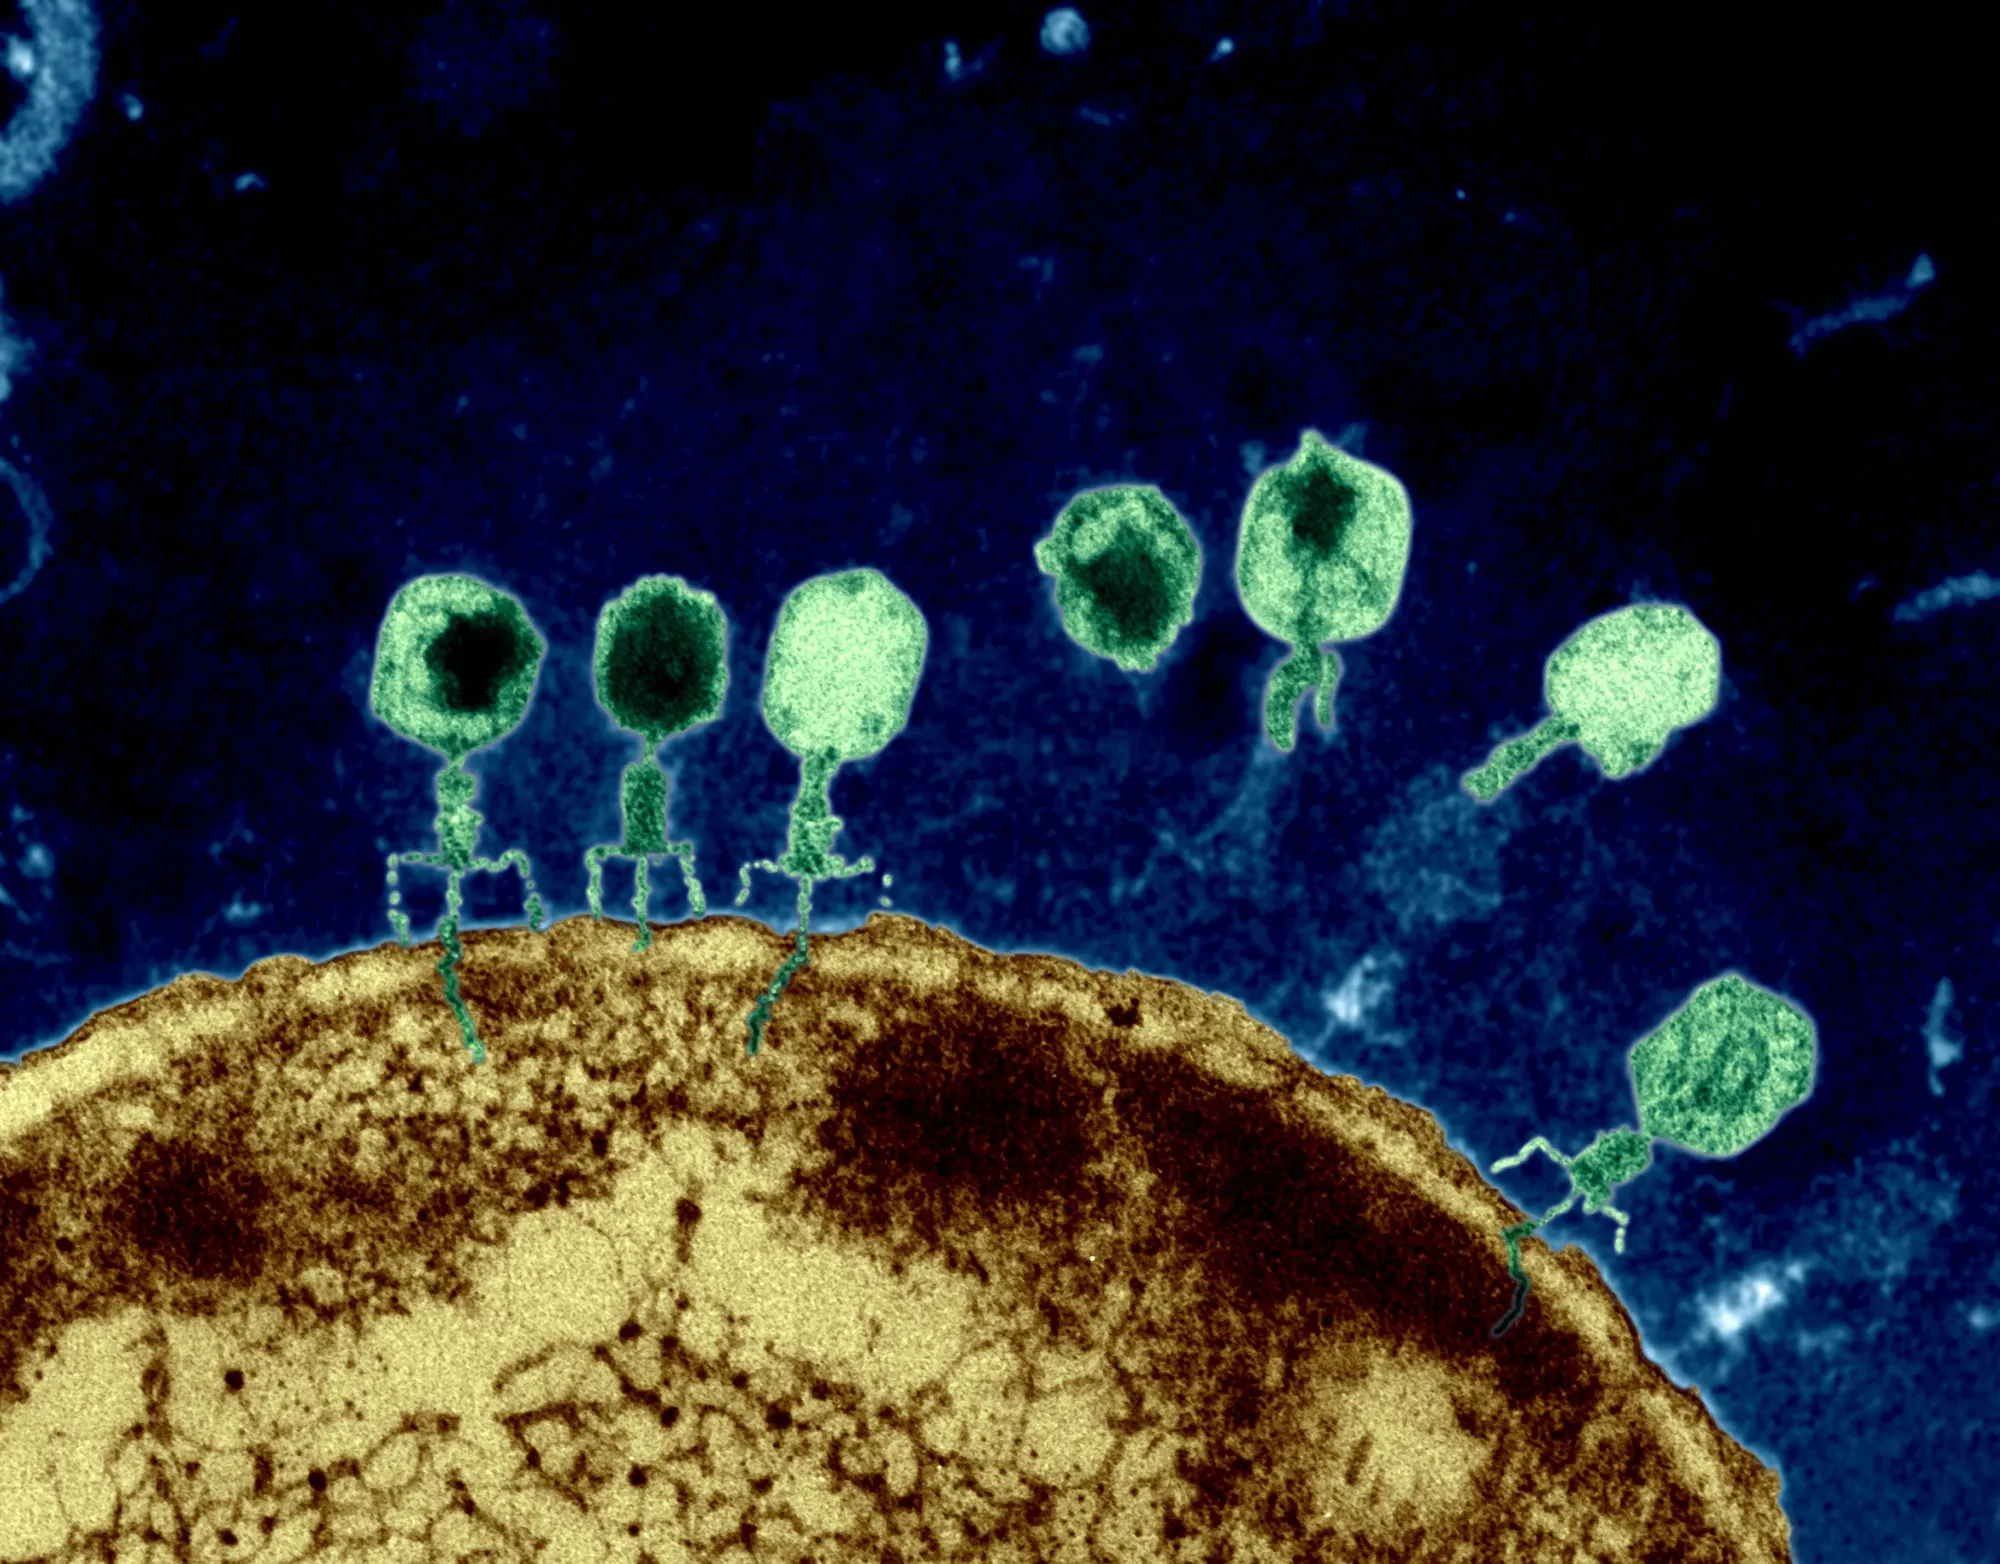
\includegraphics[width=\linewidth]{Figures/phage_real.png}
        \caption{
            Phages infecting an \textit{E. coli} bacteria. 
            % (https://www.newyorker.com/tech/annals-of-technology/phage-killer-viral-dark-matter). 
        }
        \label{fig:figures:phage_real}
    \end{subfigure}
    \hfill
    \begin{subfigure}{0.35\linewidth}
        \centering
        \captionsetup{width=1\linewidth}
        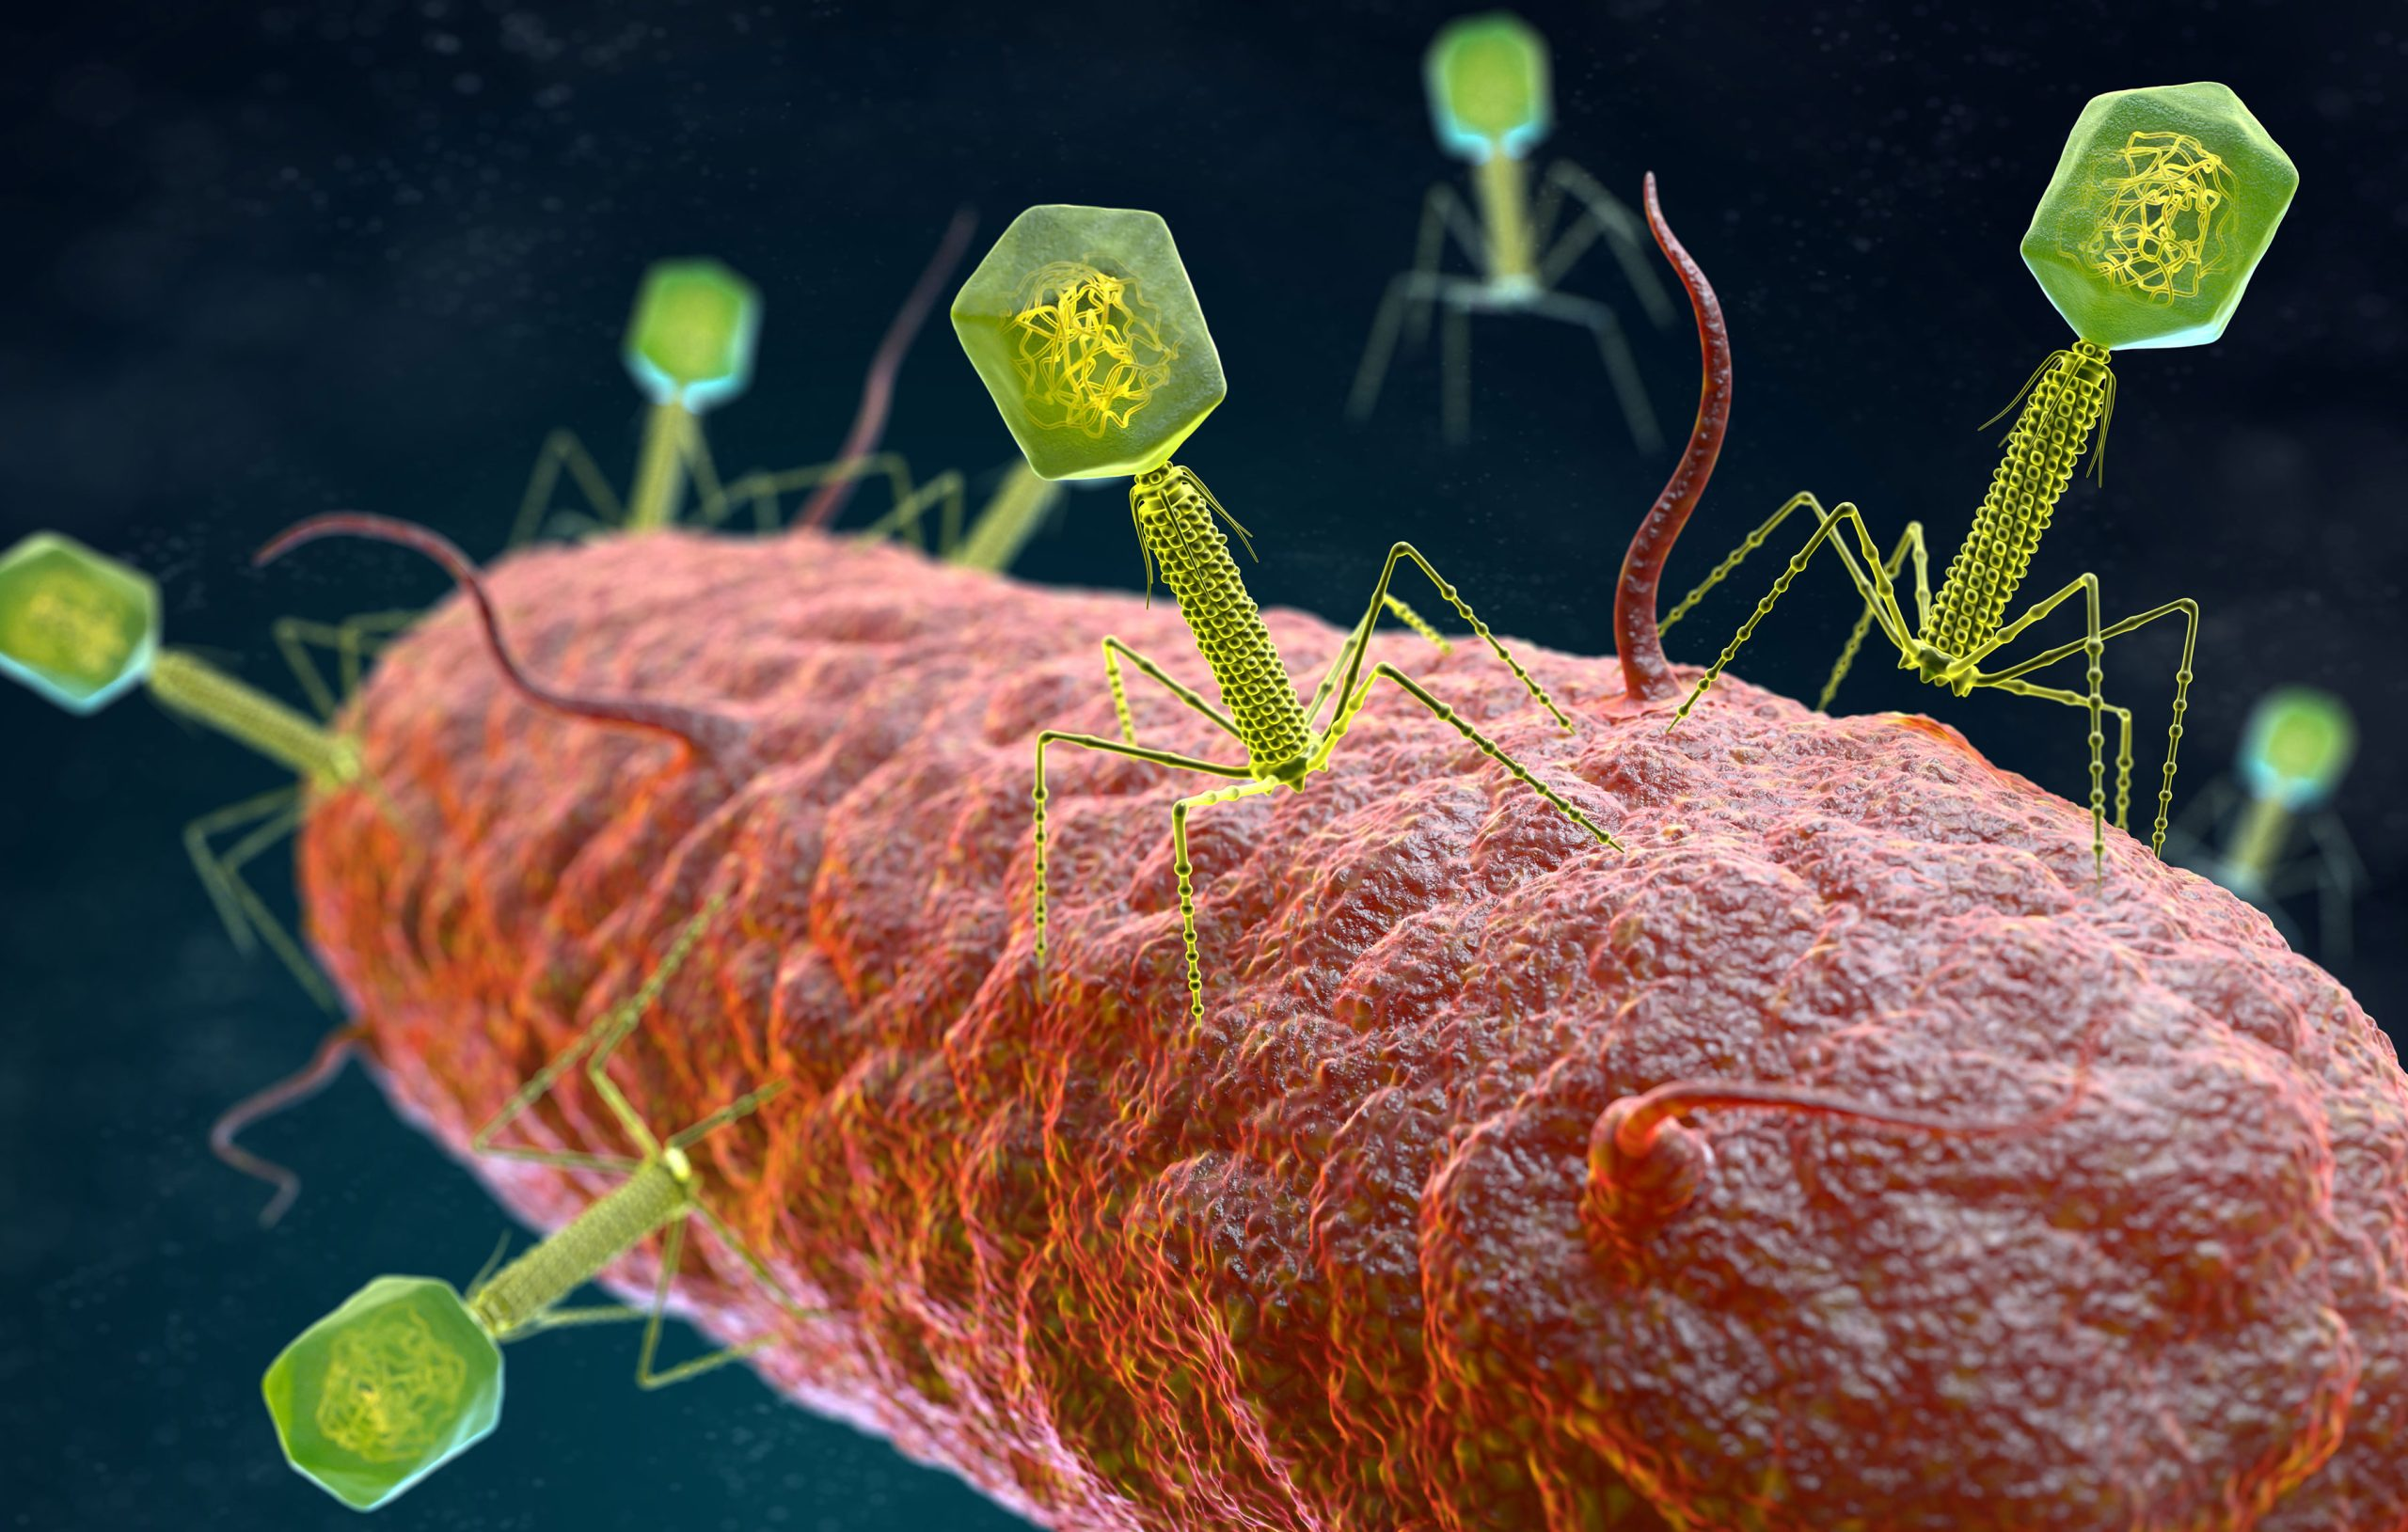
\includegraphics[width=\linewidth]{Figures/phage_impression.png}
        \caption{
            Artist representation of phages infecting a bacterium. 
            %(https://www.gettyimages.nl/detail/foto/bacteriophage-virus-attacking-a-bacterium-royalty-free-beeld/1179038792). 
        }
        \label{fig:figures:phage_impression}
    \end{subfigure}
    \caption{Parts of a phage, a real life picture of phages infecting an \textit{E. coli} bacterium, and an artist's impression of phages infecting a bacterium. }
\end{figure}

\subsection{How Does the Phage Cycle Work?}
There are 3 main parts to the phage-bacteria host cycle, the infection stage, the lysogenic cycle, and the lytic cycle. 
In the infection stage, a phage attaches to the surface of a bacteria cell. 
Once injected, the phage-cell pair can go into the lysogenic cycle or into the lytic cycle. 
\Cref{fig:phage_life_cycle} shows a detailed overview of the phage cycle. 
\newline 

In the lysogenic cycle, the phage DNA injects integrates into the genome of the bacteria. 
As the bacteria undergoes cellular replication, the DNA of the phage will be copied with the cell. 
After a set amount of time, the phage DNA can cut itself from the genome and enters the lytic cycle.
\newline 

In the lytic cycle, the phage hijacks the cellular process of the bacteria. 
The phage DNA hijacks the replication, transcription, and replication process of the cell, making more and more copies of phage. 
The phage parts build together to make a full part. 
Eventually the cell wall bursts releasing the phages into the environment ready to infect more bacteria. 

\subsubsection{Infection Stage}
The infection stage is characterized as the searching for a bacterium, detection, and subsequent attachment and injection of DNA into the bacteria. 
\paragraph{Detection and Attachment}
The phage detects the cell via phage receptor binding proteins located at the tip of the phage tail. 
The receptors are tuned to specific receptors found on the surface of the bacteria cell wall. 
Upon detection, conformational alterations in the phage's baseplate occur, causing changes in protein shapes, causing the sheath to contract and inject the viral DNA into the host. 
The successful binding and adsorption depends on the phage binding protein sensitivity, localization,and density of receptors. \cite{stoneUnderstandingExploitingPhage2019}. 
\paragraph{Phage DNA Injection}
The injection is triggered by the recognition between the phage's receptor-binding protein located at the tip of the tail and a specific receptor located on the surface of the bacteria. 
The specificity of recognition is directly related to the specificity of adsorption, which correlates to the structure of receptors located on the host's cell surface \cite{stoneUnderstandingExploitingPhage2019}. 
Once a suitable injection site has been identified, the phage injects the DNA into the cytoplasm of the cell. 
The injected DNA can replicate independently of chromosomes. 

\subsubsection{Lysogenic Cycle}
The lysogenic cycle describes the process in which the viral DNA evades detection, integrates into the cell's DNA, replicates with the cell, and cuts itself from the host's DNA to enter the lytic cycle. 
Prophages are phages that have integrated into the host's DNA. 

\paragraph{Repression of Phage DNA Detection}
Phages need to evade various cellular viral detection methods. 
CBASS triggers effector proteins that cause cell death, preventing phage replication and lysis \cite{banhBacterialCGASSenses2023}. 
Two benefits for the bacteria is that the cell death slows the growth of phages and the dead cells release resources into the environment, allowing other bacteria to recycle the resources and grow \cite{warwick-dugdaleHosthijackingPlanktonicPiracy2019}. 

% CRISPR-Cas is another method that bacteria can use to detect the presence of phage DNA. 
% CRISPR-Cas is an adaptive immune system in bacteria that defends against phages by acquiring foreign DNA sequences (spacers) into its CRISPR array, transcribing them into CRISPR RNAs (crRNAs), and using these crRNAs with Cas proteins to identify and degrade foreign DNA \cite{levyCRISPRAdaptationBiases2015}. 


\paragraph{Phage DNA Integration Into Bacteria DNA}
Phage DNA integrates into the bacterial genome as a prophage. 
This can alter host fitness by modifying metabolic pathways and cellular functions or increasing resistance to other phages, allowing the prophage to persist until conditions favor entry into the lytic cycle \cite{warwick-dugdaleHosthijackingPlanktonicPiracy2019}.

\paragraph{Cellular Replication}
The cell undergoes division multiple times, copying the prophage DNA into the cell copies. 
However prophages are still at risk of being discovered and excised by restriction enzymes \cite{sharpMolecularEvolutionBacteriophages1986}. 
\paragraph{Phage Induction}
Prophages induce (leave) from the bacteria DNA under specific conditions. 
The induction process starts with proteolytic cleavage and displacement of the phage repressor. 

This is typically seen in the lab upon activation of the SOS response following DNA damage \cite{waldorPhageRegulatoryCircuits2005}. 
Cell stressors such as DNA-damaging entities like UV light and antibiotics can jump-start the process to switch to the lytic cycle \cite{stoneUnderstandingExploitingPhage2019, fortierImportanceProphagesEvolution2013}. 

\subsubsection{Lytic Cycle}
The lytic cycle describes the process in which the viral DNA hijacks the DNA replication process, assembles within the cell, and lyses the cell releasing the phages into the environment. 
\paragraph{Hijacking DNA Replication Process}
The phage hijacks the cellular replication process to create the different proteins that make up the phage, like the long tail fiber, tail tube and sheath, and capsid \Cref{fig:figures:phage_diagram}. 
The phage redirects energy and resources from cellular functions towards viral replication \cite{warwick-dugdaleHosthijackingPlanktonicPiracy2019}. 
\paragraph{Assembly of Phage Parts}
Phage parts self-assemble by using various protein-protein and protein-nucleic acid interactions \cite{aksyukBacteriophageAssembly2011}. 
\paragraph{Lysis of the Bacterial Cell}
Many phages produce holin proteins that trigger and degrade the cell wall, releasing the phages and internally stored resources into the environment. 
Holins accumulate in the membrane until a specific time preprogrammed in the protein tells it to destroy the cell wall. 
The protein faces intense evolutionary pressure to control the length of the lytic cycle and ensure lysis at the optimal time \cite{wangHolinsProteinClocks2000}. 

\section{Bacterial Defense Against Phages} 
\label{sec:literaturereview:bacterial_defense_against_phages}
There is a constant battle between phages and bacteria. 
The bacteria don't want to be killed by the phages, so they adapt defenses such as thickening of the cell wall or destroy the viral DNA. 

\subsection{Mutations in Bacterial DNA (Genetic (Co-)Evolution)}
As bacteria cells grow and divide, random point mutations can occur in the DNA. 
These mutations can affect phage defenses, like thickening the cell wall or removing a receptor, making it harder for the phages to detect and infect the cell. 
Mutations can be partially effective if full effectiveness requires multiple steps to achieve. 
Mutations can fail or the mutation brings a cost to the bacteria cell by losing receptors on the cell wall \cite{lenskiTWOSTEPRESISTANCEESCHERICHIA1984}. 

\subsection{Horizontally Transferring DNA}
Bacteria can horizontally transfer DNA to other bacteria on contact. 
A donor cell can donate DNA fragments using a mechanism called the F-factor or plasmid with a pilus. 
The pilus acts as a tunnel between the donor cell and the recipient cell so that DNA can be transferred from the donor cell to the receiver cell. 
This method of sharing DNA can also have the unintended side effect where one bacteria will directly infect another bacteria by transferring phage DNA. 

A phage can accidentally collect a piece of the host's DNA instead of its own DNA during assembly. 
The phage with the now dead hosts DNA can infect the next bacteria, injecting the new bacterium with the dead cell's DNA, horizontally transferring the DNA \cite{tamangHorizontalGeneTransfer2023, kasmanBacteriophages2025}. 
The transferred DNA can include natural phage defenses or significantly alter the DNA of the bacterium that future phages can't detect it anymore. 

\subsection{Phage Inactivation and Decoys}
Bacteria can further protect themselves by producing decoys that the phage will attach to instead of themselves. 
Freshly lysed bacteria may still have biomarkers that attract phages, leading phages to attach to non-viable cells where successful infection cannot occur.
Bacteria can also produce proteolytic enzymes that will damage the proteins found in a phage \cite{tanQuorumSensingDetermines2015}. 
Some bacteria can produce outer membrane vesicles that phages can absorb to, and later detach and float away with the phage \cite{rabinovitchBacterialDebrisEcological2003}. 
It is suspected that the impact of these vesicles acting as a sink is minor \cite{bullPhageBacterialDynamicsSpatial2018}. 

% \subsection{CRISPR-Cas Methods}
% CRISPR is a gene editing tool that cells can use to cut out specified/unwanted parts of a DNA strand. 
% Researchers are commonly using CRISPR to genetically engineer plants and animals to have specific features. 
% Strands of DNA can be selectively added or removed from a DNA strand to achieve a better, more desired DNA strand. 
% CRISPR defenses in the bacteria can detect the unwanted phage DNA and remove the DNA. 

\subsection{Phenotype Resistance}
Not all new phenotypes arise from genetic mutations. 
Resistance can result from phenotypic variation within a genetically identical population, allowing bacteria to express different resistance traits without altering their DNA.
\citet{guptaCombinatorialPhenotypicLandscape2025} found that some \textit{Bacteroides fragilis} bacteria were able to evade phage infection.  
The presence of combinatorial phenotypic states where differential expression of protective mechanisms created rare super-resistant cells capable of withstanding phage attack.
By acting together, these heterogeneously expressed anti-phage defense mechanisms created a phenotypic landscape where distinct protective combinations enabled the survival and re-growth of bacteria expressing these phenotypes without acquiring additional mutations. 

\subsection{Spatial Refuge/Biofilms} 
Usually bacteria and phages coexist in well mixed environments such as the ocean, however some environments offer natural structures for bacteria to hide behind. 
These structures can range from physical structure, like sediment in water to biochemical structures like biofilms, where the phages can't diffuse through the biofilm. 
In large enough quantities, bacteria and other microbial communities create biofilms, a layer of mucus containing various microbes. 
The thick mucus, microbes, and other spatial effects help protect the bacteria in the biofilm from external phages by making it hard for the phages to penetrate and diffuse through the mucus \cite{abedonPhageDelayEnhancing2017}. 
In the case of a lab experiment on an agar plate, bacteria protect one another by making it harder for the phages to diffuse through the system \cite{eriksenGrowingMicrocolonyCan2018}. 

Phage movement is passive, relying on diffusion through the environment or via pressure and temperature gradients \cite{lohrmannInfluenceBacterialSwimming2024}. 
Unlike phages, bacteria possess motility, allowing them to actively move through their environment increasing their chance of survival. 

\section{Phage Counter Defense Against Bacteria}
With some of the defenses that bacteria have developed, phages are always mutating to counter their defenses. 
If phages don't adapt to the ever-changing bacterial defenses, the phages will die out due to their inability to infect and multiply. 
It essentially becomes an arms race, seeing who can out-adapt the other. 
A delicate balance therefore needs to be achieved so that both the bacteria and the phages can coexist. 

\subsection{Genetic Mutations}
Mutations in viral DNA will affect how the phage body parts are designed and built. 
These mutations will affect external phage behavior such as how it detects a bacterium, as well as internal behavior such as evading detection and integrating with the cell's DNA. 
The changes will lead to changes in overall phage fitness, ie the ability for the phage to infect, replicate, and lyse bacteria. 

\subsection{Viral Recombination}
Multiple phages can infect a cell and replicate itself using the cells internal replication process. 
Each phage has its own building blocks. 
If the proteins that build the subparts of each phage have similar chemical properties, they can be swapped between phages \cite{aksyukBacteriophageAssembly2011}. 
This allows for biological diversity to spread throughout a phage population. 
Each phage body part can have unique characteristics such as better attachment rate, larger DNA storage capsule, or better probability of injection. 


\section{Phage Defense Against Phages}
Some phages can employ defenses against other phages from infecting the bacterial cell ensuring the host resources are all for itself. 
The act of preventing a secondary infection from a similar or closely related phage is called superinfection exclusion (SIE) \cite{patelAntiphageDefenceInhibition2024}. 
There are various methods of preventing further infections that are listed below. 

\subsection{Altering Cell Structure}
The prophage can alter the surface receptors of the bacteria, making it harder for other phages to detect the bacteria, reducing the chance of attachment and injection by other phages \cite{bucherPhageMachineSIEence2024}. 

\subsection{Protein Creation}
Other phages like the T4 phage can create proteins like the Spackle protein which inhibits the lysozyme activity used in the process of DNA injection by other phages \cite{bucherPhageMachineSIEence2024, kanamaruStructureFunctionT42020}. 
Some prophages can encode proteins that will interfere with the replication process of other phages. 
For example, the SieA protein encoded by phage P22 blocks infection from other phages \cite{leavittBacteriophageP22SieAmediated2024}. 

Tail Assembly Blocker (TAB) is an anti-phage defense mechanism encoded by a \textit{Pseudomonas aeruginosa} prophage. 
While TAB permits the invading phage to replicate its genome, it inhibits the assembly of the phage tail, thereby preventing the production of infectious virions. 
The prophage that encodes TAB is not affected by this inhibition, as it also expresses a protein that neutralizes TAB's blocking activity. 
Although the host cell still undergoes lysis, no infectious phages are released.

\section{Bacteria and Phages in the Lab}
Researchers around the world are running lab experiments to gain further knowledge of the interactions between phages and bacteria. 
The aim is to better understand how phages work and interact with bacteria at a molecular, host, and population level. 

A researcher might run the experiment in a liquid medium containing water, carbon and nitrogen sources, and other chemicals such as anti-foaming or pH control chemicals. 
This liquid medium, often referred to as broth, allows for the cultivation of bacteria in a well-mixed environment, enabling researchers to monitor bacterial growth and phage infection dynamics over time. 
By adjusting parameters such as resource concentration, temperature, agitation speed, and pH, researchers can simulate different environmental conditions and observe their effects on phage-bacteria interactions. 

Samples can be taken at various time points to measure bacterial density, phage titer, and resource concentration, providing quantitative data for model validation and hypothesis testing. 
If measured frequently enough, the researcher can get an ODE-like curve out, where each datapoint represents the bacteria population level at that time. 
Researchers create a mathematical interpretation of the bacteria growth curve and run curve fitting algorithms to find the model parameters. 
The phage parameters such as latent time and burst size can be found by analyzing the phage one-step growth curve \cite{gengUsingBacterialPopulation2024, mullaExtremeDiversityPhage2024}. 

Commonly used setups include liquids containing phages, bacteria, and resources in a chemostat and batch culture. 
Chemostats allow for continuous addition of resources and removal of waste, maintaining steady-state conditions ideal for studying long-term dynamics.
Bacteria density in clear liquid mediums can be measured optically using light. 
As the bacteria grow and die, the solution will get more cloudy. 
By shining a light through a vial with bacteria growth, the change in light refraction and intensity can be measured. 
A researcher might also be interested in using a mass spectrometer to measure the density of phages and resources at specific time points. 

Petri dishes are another commonly used way to grow bacterial colonies. 
Agar, a jelly-like substance derived from seaweed, is commonly used as a solid growth medium in petri dishes. 
Agar provides a stable surface for bacteria to grow on and form visible colonies. 
Researchers can tailor the nutrients and resources in the medium to support the growth of specific bacterial strains or to test the effects of different environmental conditions. 
When phages are introduced, clear zones called plaques appear where phages have infected and lysed the bacteria, allowing for quantification and observation of phage activity. 
As a cell lyses, it releases phages into the surrounding. 
The phages can diffuse through the system, infecting neighboring cells. 
Phage infection creates clear plaques (2-3 mm) where bacteria are absent. 
See \Cref{fig:phage_petri_dish} for an example.

With petri dishes, it is harder to measure the bacterial growth. 
Bacteria are mixed with phages in a heated liquid agar solution, and poured onto a petri dish. 
It might be possible to wash the bacteria off into a container to measure the optical density (OD), but the results are not always consistent. 
Measuring OD is inaccurate and can only accurately measure up to an OD of 0.1. Even though using a special spectrophotometer allows consistent results, the results are dependent on the medium, the length of travel through the medium, bacteria size and density. 
The device and measurements need to be calibrated to ensure proper results. 
Changing methods to using $\frac{\textit{cells}}{\textit{ml}}$ instead of OD can be used to directly compare results across experiments, labs, and bacteria colonies \cite{miraEstimatingMicrobialPopulation2022}. 

A computer vision algorithm might be able to quantify the change in color on the petri dish, by comparing the photo of the bacterial lawn with a reference photo with no bacteria growth. 
The algorithm could alternatively calculate plaque sizes and determine phage concentration. 
The results are however sensitive to camera settings and external lighting changing the room brightness.  

\begin{figure}[h!]
    \includegraphics[width=0.5\textwidth]{Figures/phage_petri_dish.jpeg}
    \centering
    \caption{
        Bacteria lawn, the dots on the petri dish show no bacteria growth due to the presence of phages. 
        Photo courtesy of S. Flickinger. 
    }
    \label{fig:phage_petri_dish}
\end{figure}

\subsection{Growth Curves Typically Seen in a Lab}
\label{sec:literaturereview:growth_curves_typically_seen_in_a_lab}

When choosing parameter values it is important to choose parameter values that could realistically be found in real life systems and be replicated in the lab. 
There are various features that a researcher will be looking for in growth curve produced in a lab.
A combination of these features results in an ideal growth curve that replicates real life bacterial growth. 

The idealized dynamics of bacterial populations undergoing phage infection have several phases. First, there is a clear exponential rise in bacteria growth, and can expect to grow 40-100x in the span of a few hours. 
At a certain point in time, the bacteria population start decreasing, almost as fast as they were growing. 

Phage populations also exhibit exponential growth, but with a delay in growth. 
There is initially no growth in phage population. 
After a set amount of time, the phage population will start to grow and peak a few hours after the bacteria population reached its peak. 
If there is no phage death or removal, the phage population will eventually reach a plateau when every bacteria has died. 

\Cref{fig:created:a_good_curve_linear} shows an example of a curve for a $1\times1\times1$ system that would typically be seen in a lab. 
\Cref{fig:created:a_good_curve_logarithmic} is the same plot but with a logarithmic y-axis. 
These specific plots exhibiting a clear growth, peak, delay, and death cycle. 

\begin{figure}[h!]
    \centering
    \begin{subfigure}{1\linewidth}
        \centering
        \captionsetup{width=1\linewidth}
        \includegraphics[width=\linewidth]{Plots/Created/a_good_curve_linear.png}
        \caption{
            An example linear y-axis for a curve that researchers aim to replicate. 
        }
        \label{fig:created:a_good_curve_linear}
    \end{subfigure}
    \hfill
    \begin{subfigure}{1\linewidth}
        \centering
        \captionsetup{width=1\linewidth}
        \includegraphics[width=\linewidth]{Plots/Created/a_good_curve_logarithmic.png}
        \caption{
            The equivalent logarithmic y-axis plot for a curve that researchers aim to replicate. 
        }
        \label{fig:created:a_good_curve_logarithmic}
    \end{subfigure}
    \caption{
        Growth population of a $1\times1\times1$ system. 
        The log plot allows to see behavior happening at values approaching and to plot data on a logarithmic scale. 
        The parameters used for this plot can be found in \Cref{tab:appendixE:a_good_curve}. 
    }
    \label{fig:created:a_good_curve}
\end{figure}

\section{Software Mathematically Modelling Phages, Bacteria, and Resources}
Some software programs modelling phage-bacteria-resource interactions already exists. 
\subsection{Cocktail}
\citet{nilssonCocktailComputerProgram2022} developed Cocktail to model phage-bacteria-resource kinetics in a chemostat. 
The model assumes there is one bacteria strain that can be infected by phage A and phage B, and by both phages at the same time, phage AB. 
The model models bacterial resistance to phage A, B, and AB. 
The user can control the parameter values such as resistance rate to A, B, and AB, resource concentration and outflow, and phage adsorption rate. 
The user can also control model settings, such as if the model is deterministic or stochastic, and the step size \cite{nilssonCocktailComputerProgram2022}. 
Four sample output plots are shown in \Cref{fig:sourced:cocktail_plot}. 

\subsection{PhageDyn}
PhageDyn is a Java applet that models phage dynamics in multi-reactor industrial wastewater treatment plant models. 
PhageDyn interacts with existing GPS-X \cite{AdvancedWastewaterModelling} files to incorporate phage dynamics into models of industrial wastewater treatment plants \cite{krysiak-baltynSimulationPhageDynamics2017}. 
\citet{krysiak-baltynSimulationPhageDynamics2017} developed PhageDyn to determine how phages can reduce foaming caused by bacteria in wastewater treatment plants, another real life application of phages \cite{heardEffectFilamentousBacteria2008}. 
PhageDyn does not simulate phage dynamics on its own but rather manipulates existing files in GPS-X in order to incorporate phage dynamics in wastewater treatment plant models. 
\Cref{fig:sourced:phagedyn_plot} shows the output that PhageDyn provides. 

\subsection{Cocktail and PhageDyn Limitations}
\label{sec:literature:cocktail_and_phagedyn_limitations}
There are limitations to Cocktail and PhageDyn. 
Cocktail can model up to a $2\times 1 \times 1$ system, and is designed to model a chemostat. 
Chemostats receive a constant influx of new resources and a constant removal of medium from the chemostat. 
Cocktail's model can not be easily adapted to other models. 
The ODE model accepts inputs from a hardcoded GUI frontend. 
So any changes to the frontend or to the ODE model will require changes to the ODE model and the frontend to accept the new inputs and outputs. 
The code for Cocktail is open source, so adding new buttons and changing the model should not pose a significant challenge, but still an undertaking. 

PhageDyn works with GPS-X, a very niche wastewater treatment modelling software. 
PhageDyn is programmed for a very specific task with no flexibility in changing the model or inputs. 
PhageDyn assumes biomass, instead of individual bacteria populations. 
However, PhageDyn is no longer available for download.

\begin{figure}
    \centering
    \begin{subfigure}{0.49\linewidth}
        \centering
        \captionsetup{width=1\linewidth}
        \includegraphics[width=\linewidth]{Plots/Sourced/cocktail_plot.png}
        \caption{
            Figure A) \textit{E. coli} infected with phage T4 in a chemostat exhibiting an oscillating growth behavior, following the model of \citet{bohannanEffectResourceEnrichment1997}. 
            Figure B) Oscillations of bacteria and phages can exist at higher titers, dependent on low resource concentration, following the model of \citet{lenskiDynamicsInteractionsBacteria1988}. 
            Figure C) As the concentration of resources change, this results in increasing oscillations, but not going extinct. 
            Figure D) A system modelling the interactions with phage A and B. 
        }
        \label{fig:sourced:cocktail_plot}
    \end{subfigure}
    \hfill
    \begin{subfigure}{0.49\linewidth}
        \centering
        \captionsetup{width=1\linewidth}
        \includegraphics[width=\linewidth]{Plots/Sourced/phagedyn_plot.png}
        \caption{
            \textcolor[HTML]{551A8C}{\textbf{Purple}} is heterotrophic biomass, 
            \textcolor[HTML]{4580B4}{\textbf{Blue}} is foaming biomass, 
            \textcolor[HTML]{FF0000}{\textbf{Red}} is phages, 
            \textcolor[HTML]{01E6EE}{\textbf{Light Blue}} is total suspended solids. 
            Figure A) Biomass concentration immediately post phage dosing. 
            Figure B) Biomass concentration with low phage concentration and maintain low concentration post spike in population count. 
            Figure C) Biomass concentration when phages are extinct. 
            Figure D) Biomass concentration with a less virulent and low adsorption rate phage, co-existence with biomass reached. 
            A change in phage concentration shows a decrease in heterotrophic and foaming biomass \cite{krysiak-baltynSimulationPhageDynamics2017}. 
        }
        \label{fig:sourced:phagedyn_plot}
    \end{subfigure}
    \caption{Example output from Cocktail and PhageDyn respectively. For PhageDyn, concentration of heterotrophic biomass in an aerobic plug flow across four situations.
        See \citet{nilssonCocktailComputerProgram2022} and \citet{krysiak-baltynSimulationPhageDynamics2017} for more information on parameter values and supplementary resources. 
    }
    \label{fig:sourced:cocktail_and_phagedyn}
\end{figure} %Related literature and material (8-12 pages)
\newpage

\lhead{\emph{Methods}}
\chapter{Methods}
\label{Methods}
\section{Project Overview}
To help complete this Master thesis, I created various tools that would help create the final model outputs.
The project is divided into three logical parts, with an optional fourth part.


\subsection{Part 1: Network Creation Tool (GUI)}
\label{sec:part1}
The first part involves the development of a GUI tool to create and edit the network topography of interactions.
This tool allows users to quickly and intuitively define agents, interaction parameters, environmental parameters, and setting parameters.
The tool provides functionalities for adding, editing, and visualizing nodes and edges, as well as importing and exporting the network structure. \newline 
Once the user is happy with the graph shape, they can export the graph for use in part 2 (\Cref{sec:part2}), part 3 (\Cref{sec:part3}), and part 4 (\Cref{sec:part4}). 
The most important part is that the user defines the network edges and the attributes that each node and edge has, as that can't be edited in part 2 onwards. 
It's not a big issue however because the user can upload the graph to the tool again to edit the edge connections and add or remove nodes and attributes. 
In part 3, the user can edit the values of the attributes, so the parameter values do not have to be dialed in, and the user does not need to use the GUI tool to edit parameter values. 


\subsection{Part 2: Simulation Framework}
\label{sec:part2}
The second part focuses on the simulation framework.
The user provides an ODE model and the network topography as input to the framework.
The simulation framework deals with handling the input and output of the data, collecting and storing the data needed for the simulation.
The framework uses SciPy's \textit{solve\_ivp()} numerical solver to simulate the provided ODE equations and calculate the population levels through time.
As output, the user receives two outputs.
The first output is an array of time values that the solver used to calculate the population count.
The second output is an array containing the population count at each time step for every agent.


\subsection{Part 3: Analysis and Visualization}
\label{sec:part3}
The third part involves analyzing and visualizing the simulation results.
The user can use a dashboard built using Plotly Dash to interact with the solver and network.
The user can change parameter, environment values, and setting values on the fly.
This allows the user to quickly change parameter values and test different situations.
The dashboard includes various starter plots that allow the user to test the model.


\section{Part 4: Network Topography of Interactions Creation Tool}
\label{sec:part4}
In a microbial environment, numerous interactions are occurring between agents.
However, not every agent can and will interact with one another.
Based on which agents interact with one another, a network topography can be created, capturing the dynamics of the interactions.
Every node represents a unique agent.
An edge links agents together if there is an arbitrary interaction occurring between the agents. 
The network allows for self-loops.


Each node contains attributes and properties intrinsic to that agent.
For example, this would include the starting population or concentration, reproduction speed (if any), or death rate (if any).
Each edge likewise also contains attributes to capture the unique dynamic interactions between the agents.
This could be the probability for a successful interaction, the burst size of a specific phage-bacteria pair, or the bacteria's consumption rate of resources.
Adding the attributes to the nodes and edges allow for the capture of various interaction dynamics within the context of the community.
The interactions between the agents can be visualized and edited using a GUI tool.


A GUI tool has been developed using Python and NetworkX to help aid in the development of this network topography.
With this tool, a network topography can be created by adding any number of agents of varying types, such as bacteria, phages, or resources.
There is an environment node that is used to store global environmental data, for example, the temperature of the system, the pH of the system, the wash-in/out rate, etc.
There is a settings node that holds information such as simulation length, max time step, and the type of ODE solver to use.
The attributes of the agents, interactions, and environment can easily be edited using the GUI tool.

\Cref{fig:ss:initial_startup_GUI_tool} shows the layout of the GUI tool built using Tkinter and NetworkX. \Cref{fig:ss:example_network} shows an example network that can be created. %TODO: Citation needed.
There are numerous buttons that can be used to edit the graph, for example adding or removing nodes and edges. 
By default, an environment node holding parameters such as pH and temperature is added.
A settings node is added as well, holding settings data to be used for the solver, like the type of solver or simulation length.
Manually adding nodes and edges can get tedious and repetitive for large graphs, so the user can add multiple nodes and edges at the same time.
Nothing can interact with the environment and setting node, as they are used to hold data about the environment and network solver.
For each node and edge, default attribute names and values are added which can later be edited by the user. 
The user can alter the default attribute name and value by importing the GUI tool class and overriding the method implementation implementing the default names and values. 
The nature of the interaction needs to be defined and captured in the parameter names, values, and ODE equations.

\begin{figure}
    \centering
    \begin{subfigure}{0.49\linewidth}
        \centering
        \vspace*{\fill}
        \includegraphics[width=\linewidth]{Screenshots/initial_startup_GUI_tool.png}
        \caption{
            The GUI tool as seen on the startup of the program.
        }
        \label{fig:ss:initial_startup_GUI_tool}
        \vspace*{\fill}
    \end{subfigure}
    \begin{subfigure}{0.49\linewidth}
        \centering
        \vspace*{\fill}
        \includegraphics[width=\linewidth]{Screenshots/example_network.png}
        \caption{
            An arbitrary $3\times2\times3$ network with each node representing a phage, bacteria, or resource, with arbitrary interactions occurring between them. 
        }
        \vspace*{\fill}
        \label{fig:ss:example_network}
    \end{subfigure} 
 \end{figure}

\section{Dashboard for Analysis and Visualization}
The dashboard allows the user to interact with the network, the model, and some prebuilt visualizations, and is built into three logical sections.
The first section allows for the user to edit the network parameters and setting values on the fly to quickly iterate through different conditions and to fine-tune parameter selection without having to rebuild the network using the GUI tool.
The second section allows for the user to see how the population count evolves over time for a given initial condition and parameter values, allowing to quickly test the network input.
The final section allows for the user to run more advanced analyses on the network, for example, by changing multiple parameter values and visualizing the output. 

\subsection{Editing Network and Parameter Values}
\label{sec:editing_network_and_parameter_values}
The editing network and parameter value contain five separate sections.
\subsubsection{Initial Condition}
The initial condition settings panel (\Cref{fig:ss:ds:initial_condition}) allows for the user to edit the initial starting values of the agents. 
Each agent type has a table containing the initial population count. 
An extra hidden agent can be included. 
When a bacteria has been infected, the bacteria goes through multiple stages before lysing. Each bacteria agent starts out as uninfected, and once infected, the bacteria goes through 4 stages of infection before lysing as seen in \Cref{fig:ss:ds:initial_condition}. \newline 
Data that can be represented as a vector, for example the data attributed to an agent type have their own section, \Cref{fig:ss:ds:vector}.
Data that is stored as a matrix, the data stored on edges between agents, is stored in the matrix tab (\Cref{fig:ss:ds:matrix}).
The environment data and settings data also have their own tab, \Cref{fig:ss:ds:environment} and \Cref{fig:ss:ds:settings} respectively.

\begin{figure}[h!]
    \centering
    \begin{subfigure}{0.49\linewidth}
        \centering
        \vspace*{\fill}
        \includegraphics[width=\linewidth]{Screenshots/DashboardSettings/initial_condition_settings.png}
        \caption{
            The tab where the user can edit the initial conditions of the agents.
        }
        \label{fig:ss:ds:initial_condition}
        \vspace*{\fill}
    \end{subfigure}
    \hfill
    \begin{subfigure}{0.49\linewidth}
        \centering
        \vspace*{\fill}
        \includegraphics[width=\linewidth]{Screenshots/DashboardSettings/initial_matrix_settings.png}
        \caption{
            The tab where the user can edit the matrix attribute values. 
        }
        \label{fig:ss:ds:matrix}
        \vspace*{\fill}
    \end{subfigure}
    \hfill
    \begin{subfigure}{0.49\linewidth}
        \centering
        \vspace*{\fill}
        \includegraphics[width=\linewidth]{Screenshots/DashboardSettings/initial_vector_settings.png}
        \caption{
            The tab where the user can edit the vector attribute values.
        }
        \vspace*{\fill}
        \label{fig:ss:ds:vector}
    \end{subfigure}
    \hfill
    \begin{subfigure}{0.49\linewidth}
        \centering
        \vspace*{\fill}
        \includegraphics[width=\linewidth]{Screenshots/DashboardSettings/initial_environment_settings.png}
        \caption{
            The tab where the user can edit the environment values. 
        }
        \label{fig:ss:ds:environment}
        \vspace*{\fill}
    \end{subfigure}
    \hfill
    \begin{subfigure}{0.49\linewidth}
        \centering
        \vspace*{\fill}
        \includegraphics[width=\linewidth]{Screenshots/DashboardSettings/initial_settings_settings.png}
        \caption{
            The tab where a user can edit the settings of the solver and simulation. 
        }
        \label{fig:ss:ds:settings}
        \vspace*{\fill}
    \end{subfigure}
    \caption{The tabs where the user can edit the various parameter values and control the simulation parameters}
 \end{figure}

\subsection{Advanced Visualization and Analysis}
In the advanced analysis section, the user can run different analysis methods to gain a greater understanding of the model.
The visualizations only support a $1 \times 1\times 1$ model, in order to make the analysis easier for the user, and to make it easier to analyze the visualization.
These advanced visualizations were created with the mind of understanding a simple network.
There are five different analysis and visualization methods, and one system where the user can run a large simulation on the whole network and receive an output file containing the raw simulation file data.
The raw data is stored as a \textit{parquet} file, a tabular-like data format, which when combined with Dask (not Dash), allows for querying of the data similarly to Pandas.
Parquet with Dask offers superior performance and data storage solutions that Pandas can't offer.
Once queried, the user can create their own graphs and plots as they have access to the parameter values used and the raw simulation data.

\subsubsection{Serial Transfer}
Serial transfer is a method employed by bacteriologist where after a set amount of time, the bacteriologist pipettes a specified amount of media (for example 10ml of liquid) containing bacteria and nutrients, possibly with phages, and transfers the old media into a solution containing new media.
At this stage, the bacteriologist can introduce new agents, or re-introduce agents if the agent population or concentration has died out.
However, usually only resources are added during the transfer process.
An example would be an experiment starts with 50ml of solution.
The experiment runs for 24 hours before 5ml is removed.
Researchers can run various tests, such as using optical density measurements to assess bacterial density in the solution or employing a mass spectrometer to determine the concentration of the resources.
The 5ml is then re-added to a new solution of 45ml containing fresh resources.
The effect that this has is it creates a sort of artificial stable point.
As the bacteria grow, they consume the resources found in the solution.
However eventually the resources run out, and the bacteria die out due to a lack of nutrients.
By introducing new nutrients at set time intervals, the bacteria can regrow and exhibit a semi-stationary behavior.
\newline

The implementation of serial transfer is slightly different.
A user can select a number which will divide the population count of the agents by that number (\Cref{fig:ss:av:serial_transfer_settings}).
Then the program takes the initial condition values defined for the nutrients the initial condition in \Cref{sec:editing_network_and_parameter_values} and adds those values to the nutrients respectively.
By selecting a checkbox, the values as defined in the initial condition box for phages and bacteria in \Cref{sec:editing_network_and_parameter_values} can optionally be added as well.
As an example, if at the end of a simulation, there are 120 resources, 5000 bacteria, and 1000 phages remaining and the chosen serial transfer value is 15, then the resource, bacteria, and phage values would be decreased to 8, 333.33, and 66.66 respectively.
Then, if the initial condition for the resources, bacteria, and phages in \Cref{sec:editing_network_and_parameter_values} are 500, 80, and 10 respectively, and the checkbox is unchecked, the new population count will be 508, 333.33 and 66.66 respectively.
If the checkbox is checked, the new population count will be 508, 413.33, and 76.66 respectively.
These new values would be used as the new starting initial condition for a new simulation, and the run results will be appended to the previous run.
As output, new graphs are created showing the runs appended to one another, with an example output shown in \Cref{fig:ss:av:serial_transfer_run}.

\begin{figure}[h!]
    \centering
    \begin{subfigure}{0.49\linewidth}
        \centering
        \vspace*{\fill}
        \includegraphics[width=\linewidth]{Screenshots/AdvancedVisualization/serial_transfer_settings.png}
        \caption{
            The section where the user can set up the serial transfer.
        }
        \label{fig:ss:av:serial_transfer_settings}
        \vspace*{\fill}
    \end{subfigure}
    \hfill
    \begin{subfigure}{0.49\linewidth}
        \centering
        \vspace*{\fill}
        \includegraphics[width=\linewidth]{Screenshots/AdvancedVisualization/serial_transfer_run.png}
        \caption{
            The output plots of serial transfer. 
        }
        \label{fig:ss:av:serial_transfer_run}
        \vspace*{\fill}
    \end{subfigure}
    \caption{Serial Transfer}
 \end{figure}

\subsubsection{Parameter Analysis}
The parameter analysis settings tab as shown in \Cref{fig:ss:av:parameter_analysis_settings} allows the user to choose two parameters and individually run the model with the varying input values.
The values that can be tested and changed include all initial condition values, vector and matrix data, and environmental data.
As input, the user can select 2 parameters of choice.
After the parameter name selection, the user can manually choose which parameter values they want to test or test a range of values equally spaced by selecting the number of values to test.
Finally, the user can optionally run a serial transfer, where the serial transfer uses the settings found on the Serial Transfer tab. \newline

\Cref{fig:ss:av:parameter_analysis_run} shows the heatmap that the user can expect, one heatmap for each agent type.
Each heatmap has cells that unique model input, and contains the value of
A heatmap matrix is created for each agent type, with dimension of the input values.
Each box corresponds to each pair of parameter inputs, and shows the population count of the agent at the time selected on the slider. 
As the user slides the slider, the value inside the cell changes to correspond with the chosen time. 
Note that the heatmap color range resets for each heatmap, so similar colors across heatmaps will not correspond to the same values.

\begin{figure}[h!]
    \centering
    \begin{subfigure}{0.49\linewidth}
        \centering
        \vspace*{\fill}
        \includegraphics[width=\linewidth]{Screenshots/AdvancedVisualization/parameter_analysis_settings.png}
        \caption{
            The options available for the parameter analysis. 
        }
        \label{fig:ss:av:parameter_analysis_settings}
        \vspace*{\fill}
    \end{subfigure}
    \hfill
    \begin{subfigure}{0.49\linewidth}
        \centering
        \vspace*{\fill}
        \includegraphics[width=\linewidth]{Screenshots/AdvancedVisualization/parameter_analysis_run.png}
        \caption{
            The output that the user can expect
        }
        \label{fig:ss:av:parameter_analysis_run}
        \vspace*{\fill}
    \end{subfigure}
    \caption{Parameter Analysis}
\end{figure}


\subsubsection{Initial Value Analysis}
The initial value analysis settings tab as shown in \Cref{fig:ss:av:initial_value_analysis_settings} allows the user to choose a single parameter and vary the value of that parameter, visualizing how a change in parameter value affects the population count of the agents.

\Cref{fig:ss:av:initial_value_analysis_run} shows the plots that the user receives.
For each agent type, there are three plots made.
The left plot shows the population count through time, one line for each parameter value submitted.
The middle plot takes each run and calculates the “percentage from the max value“ (default value of $0.95 \rightarrow 95\%$) reached of the peak.
This value is considered the time of peak, and is used to fix some issues that can arise where the population plateaus or only keeps on rising.
The initial value is plotted on the x-axis, with the time at which the max value is reached on the y-axis.
Using the plotted data, a linear or log fit can be created.
Using this data can be useful for understanding how a change in parameter value affects the time at which the population count reaches a maximum.
The slope, intercept and $R^2$ value is stored and saved in the third plot, a bar chart, with an editable name.
For every re-run of the initial value analysis, the slope, intercept and $R^2$ value is stored in the bar chart, allowing comparison of the slope-intercept data across different parameters. 

\begin{figure}[h!]
    \centering
    \begin{subfigure}{0.49\linewidth}
        \centering
        \vspace*{\fill}
        \includegraphics[width=\linewidth]{Screenshots/AdvancedVisualization/initial_value_analysis_settings.png}
        \caption{
            The settings for the initial value analysis tab. 
        }
        \label{fig:ss:av:initial_value_analysis_settings}
        \vspace*{\fill}
    \end{subfigure}
    \hfill
    \begin{subfigure}{0.49\linewidth}
        \centering
        \vspace*{\fill}
        \includegraphics[width=\linewidth]{Screenshots/AdvancedVisualization/initial_value_analysis_run.png}
        \caption{
            An example initial value analysis output. 
        }
        \label{fig:ss:av:initial_value_analysis_run}
        \vspace*{\fill}
    \end{subfigure}
    \caption{Initial value analysis}
\end{figure}

\subsubsection{Phase Portrait}
The phase portrait plot allows for the user to analyze how an agent population evolves with respect to the other agent population through time.
Phase portraits indicate how one population increases while the other decreases, and vice versa.
Steady states can be identified and classified as either stable, unstable, or as saddle points.
By comparing different starting points, it is possible to see if the system is chaotic or not.
The setup for the phase portrait can be seen in \Cref{fig:ss:av:phase_portrait_settings}, and a sample output can be seen in \Cref{fig:ss:av:phase_portrait_run}. 

\begin{figure}[h!]
    \centering
    \begin{subfigure}{0.49\linewidth}
        \centering
        \vspace*{\fill}
        \includegraphics[width=\linewidth]{Screenshots/AdvancedVisualization/phase_portrait_settings.png}
        \caption{
            The user can select two starting values for the initial condition, but they can't choose vector, matrix, or environment settings due to the plot showing the development of agent populations against other agent populations.
            As typical, the user can select their own values or auto-generate values between two values, as well as use a serial transfer option.
            There is also an option to take the logarithm of the x and/or y-axis. 
        }
        \label{fig:ss:av:phase_portrait_settings}
        \vspace*{\fill}
    \end{subfigure}
    \hfill
    \begin{subfigure}{0.49\linewidth}
        \centering
        \vspace*{\fill}
        \includegraphics[width=\linewidth]{Screenshots/AdvancedVisualization/phase_portrait_run.png}
        \caption{
            An example run of a phase portrait.
        }
        \label{fig:ss:av:phase_portrait_run}
        \vspace*{\fill}
    \end{subfigure}
    \caption{Phase Portrait}
\end{figure}

\subsubsection{SOBOL Analysis}
SOBOL analysis, a variance-based sensitivity analysis, is a method that allows a user to quantify how important an input parameter has on a measured aspect of the output by changing the parameter values of the model and measuring the change in model output.
SOBOL quantifies how much variance in the output can be attributed to a specific parameter and can measure the effect of global, first, and second order sensitivity. 
When a model is viewed as a black-box model, the model can be seen as a function $Y=f(X)$, where $X$ is an input vector of $d$ elements, and $Y$ is a univariate model output.
$X$ is assumed to be independently and uniformly distributed within a hypercube $X_i \in [0, 1]$ for $i=1, \dots d$.
The first order sensitivity measures the output variance of the main affect of parameter $X_i$.
Measuring the effect of varying $X_i$ averaged over other input parameters, and standardized to provide a fractional contribution to the overall output variance.
The first order sensitivity is described as
\[
    S_i = \frac{V_i}{\textit{Var}(Y)}
\] where $V_i = \textit{Var}_{X_i}(E{X_{\sim i}}(Y|X_i))$ and where $X_{\sim i}$ represents all the parameters that are not $X_i$.
\newline


The second order index measures the impact of input $X_i$ interacting with $X_j$. For many inputs, this becomes unwieldy to analyze.
The global sensitivity is used to analyze the global sensitivity without evaluating $2^d-1$ indices, and measures the contribution to the output variance of $X_i$, including all variance due to $X_i$s interaction with other variables.
\[
    S_{T_i} = \frac{E_{X_{\sim i}}(\textit{Var}_{X_i}(Y|X_{\sim i}))}{\textit{Var}(Y)} = 1 - \frac{\textit{Var}_{X_i}(E_{X_i}(Y|X_{\sim i}))}{\textit{Var}(Y)}
\]
SOBOL can analyze various univariate outputs.
This could be either the average value of an agent population, the variance in population count, the time at the peak of an agent count, the final population value, etc. \newline
SOBOL accepts a list of parameter names and a list of range of values to sample from, which the user can input in the SOBOL settings tab, \Cref{fig:ss:av:SOBOL_analysis_settings}. 
If no values are added, the parameter is not included in the simulation and the default value is instead used. 
The user then needs to select the number of samples to run, using the formula $2^x$, where $x$ is the number they input, and $2^x$ is the number of samples that SOBOL will create and run.
The larger $x$ is, the more accurate the SOBOL analysis results will be, but the more simulations would need to be run. \newline
If the user wants to analyze the second order interactions, then the model will run the system $N(2D+2)$ times with the randomly sampled input values, where $N$ is a multiple of 2, and $D$ is the number of parameters being tested.
Otherwise, if 2nd order is not chosen, the model is run $N(D+2)$ times.
Due to the randomness of the sampling method, the user can, but does not need to, submit a seed value. 


Three SOBOL analyses are included by default in the dashboard, as shown in \Cref{fig:ss:av:SOBOL_analysis_run}.
An analysis of the final value of the simulation, the average population count, and the variance in population count.
The global and first sensitivity are shown next to one another, and each sub-row within a plot represents each agent type. 
The proportion of the global and local sensitivity can be seen for each agent type and each parameter.

\begin{figure}[h!]
    \centering
    \begin{subfigure}{0.49\linewidth}
        \centering
        \vspace*{\fill}
        \includegraphics[width=\linewidth]{Screenshots/AdvancedVisualization/SOBOL_analysis_settings.png}
        \caption{
            The SOBOL settings tab. 
        }
        \label{fig:ss:av:SOBOL_analysis_settings}
        \vspace*{\fill}
    \end{subfigure}
    \hfill
    \begin{subfigure}{0.49\linewidth}
        \centering
        \vspace*{\fill}
        \includegraphics[width=\linewidth]{Screenshots/AdvancedVisualization/SOBOL_analysis_run.png}
        \caption{
            The output that can be expected from SOBOL. 
        }
        \label{fig:ss:av:SOBOL_analysis_run}
        \vspace*{\fill}
    \end{subfigure}
    \caption{SOBOL variance analysis}
\end{figure}

\subsubsection{Ultimate Analysis}
\label{sec:ultimate_analysis}
The Ultimate Analysis section does not produce any visualizations or analysis, but instead allows for the user to define which initial conditions and parameter values they want to run a simulation on.
The solver will iterate over every single parameter input possibility and save the results in a \textit{.parquet} file.
Similarly to the other sections, the user can specify a start and end value, along with the number of values to generate evenly spaced within that range, including both the start and end values.
\newline
Using Dask and the saved \textit{.parquet} file, the user can query for specific runs, for example runs where a parameter value was greater than 0.05, and use the simulation data to create their own plots.
\begin{figure}
    \centering
    \includegraphics[width=1\linewidth]{Screenshots/AdvancedVisualization/ultimate_analysis_settings.png}
    \caption{
        The ultimate analysis setup tab. 
    }
    \label{fig:ss:av:ultimate_analysis_settings}
\end{figure}


\section{Custom Advanced Analyses and Visualizations}
As the dashboard can not create a graph for every situation, or analyze every situation, Ultimate Analysis (\Cref{sec:ultimate_analysis}) can be used to run and download the simulation data to the disk to create later create your own custom visualizations. 
Depending on the used model, different behavior might appear, for example the population count can exhibit cyclic behavior. 
A custom visualization would then perform a Fourier transformation to obtain the predominant frequencies. 

\section{The Golden Model}
In this report, the default model, called the “Golden model“ \cite{gengUsingBacterialPopulation2024} that will be used for all simulations is as follows:

\begin{align}
    \frac{dN}{dt} &= -e \cdot g(N)\cdot (U + \sum_{i=1}^{M} I_M)\\
    \frac{dU}{dt} &= g(N)\cdot U - r\cdot U \cdot P\\
    \frac{dI_1}{dt} &= r\cdot U \cdot P - \frac{M}{\tau}\cdot I_1 \\
    \frac{dI_k}{dt} &= \frac{M}{\tau}(I_{k-1}-I_k) \text{ for } k=2, \dots, M \\
    \frac{dP}{dt} &= B\cdot\frac{M}{\tau} \cdot I_M - r\cdot(U + \sum_{i=1}^{M} I_M)\cdot P \\
    g(N) &= \frac{v\cdot N}{N + K}
\end{align}where $N$ is nutrients, $U$ is uninfected bacteria, $I_{1, \dots, M}$ is the infected stage of the bacteria, and $P$ is the phage population. \newline
The model describes three biological processes, cell consumption of resources and growing, phage/cell encounters and infection, and cell lysis. 
The cell growth process is described by $g(N)$, the instantaneous growth rate dependent on the Monod equation, where $v$ is the maximal growth rate and $K$ is the Monod constant. 
The consumption rate of a resource by a bacteria is $e$. \newline
Once infected by a phage, cells go through $M$ stages of infection $I_1, \dots, I_M$ before lysing, with equal transition probability $\frac{M}{\tau}$ from state $I_k$ to state $I_{k+1}$. The probability of a successful infection of a cell is $r$. \newline
After a bacteria lyses after stage $I_M$, $B$ phages are releases, the burst size of the phage. \newline 

However this model is specifically designed for a $1\times 1 \times 1$ model. 
In order to adapt this model to fit an $p \times b \times r$ model, the model needs to be adapted. 
There are other changes that can be made, to the model, for example by adding a washin rate $w^{i}$, where resources are constantly being introduced,such as in a chemostat, and a washout rate $w^{o}$ where phages, bacteria, and resources are being washed out. 

\subsection{The Golden Model Adapted}
\begin{align}
    \frac{dN_n}{dt} &= -e_{[n, b]} \cdot g(N_n)\cdot (U + \sum_{i=1}^{M} I_M)\\
    \frac{dU_b}{dt} &= g(N_n)\cdot U_b - U_b \cdot (\sum_{p \in P} r_{[p, b]} \cdot P_p)\\
    \frac{dI_{1_b}}{dt} &= r\cdot U \cdot P - \frac{M}{\tau}\cdot I_1 \\
    \frac{dI_{k_b}}{dt} &= \frac{M}{\tau}(I_{k-1}-I_k) \text{ for } k=2, \dots, M \\
    \frac{dP_p}{dt} &= B\cdot\frac{M}{\tau} \cdot I_M - r\cdot(U + \sum_{i=1}^{M} I_M)\cdot P \\
    g(N_n) &= \frac{v_\cdot N}{N + K}
\end{align}, %Details of your approach (10-15 pages)
\newpage

\lhead{\emph{Experiments and Results}}
\input{Chapters/ExperimentsandResults} %Evaluation/testing of your hypothesis (10-15 pages)
\newpage

\lhead{\emph{Discussion}}
\chapter{Discussion}
\label{Discussion}
This section presents an analysis and discussion of the results. 

\section{Graph Behavior}
\Cref{tab:results:graph_behavior} presents illustrative examples rather than a comprehensive analysis. 
The behaviors shown represent typical trends observed when varying each parameter in the specified direction, but they may not apply to all possible values or reflect the magnitude of changes. 
Additionally, these results do not necessarily generalize to scenarios where two parameters are simultaneously varied. 
\Cref{tab:results:graph_behavior} should be interpreted alongside the local $S1$ sensitivities from \nameref{sec:SOBOL_sensitivity_analysis_results} to better understand how sensitive the output is to specific parameters and the potential impact of their variation.

\section{A Good Curve}
As the bacterial population grows, resource consumption accelerates until only trace amounts remain at $t=8$. 
The delay between the peaks of uninfected and infected bacteria is due to the infection stages and the latent period of phage infection. 
Each bacterium progresses from infection stage $k$ to $k+1$ at a rate of $\frac{M}{\tau}$. 
Therefore, decreasing the number of infection steps $M$ or increasing the latent period $\tau$ amplifies this delay. 
A longer latent period means it takes more time for bacteria to progress through the infection stages.

At $t=4$, the infection rate surpasses the bacterial replication rate, causing the bacterial population to decline even though resources are still available. 
This moment coincides with the rise of the phage population. 
Observing the timing of these events and changes in graph behavior, as well as their relationships across different graphs, helps clarify the complex population dynamics and the interdependence of the populations that might not be obvious from reading the ODE model. 

This becomes more difficult when the model goes from a $1\times1\times1$ system to a $p\times b \times r$ system. 
Now up to any number of phages can interact with any number of bacteria, and any number of bacteria can interact with any number of resources at varying rates. 
These varying rates will significantly influence the dynamics of the system, and make it hard to determine what event caused what due to the rise in number of interactions.
For a $1\times1\times1$ system, there are 2 interactions that can occur (assuming no self interactions, and that phages don\t interact with the resources). 
With a $p\times b\times r$ system, there are $\mathcal{O}(p\cdot b + b\cdot r)$ interactions that can occur. 
So for a $3\times2\times3$ system, there are at most 12 interactions occurring. 
12 events can occur at the same time, making it hard to identify the cause of the event. 

\section{SOBOL Sensitivity}
SOBOL, when mixed with a qualitative analysis can provide insight into why when a parameter changes, the output changes as it does. 
A mathematician or biologist might look at an ODE model and reason through the changes. 
They might explore the model by having an internal monologue as follows. 
“If I increase $\tau$, which means that the bacteria infection process takes longer, then when a phage infects a bacterium, it will take longer for the bacteria to die. 
Dying later means that the phages are released later. 
By releasing later, it will take longer for the phages to grow and peak. 
It also allows more time for the uninfected bacteria population to grow and use up the resources. 
There will be a natural delay in uninfected bacteria peak as it takes longer for the bacteria to become infected and go through the infection process.”
\Cref{tab:results:graph_behavior} aims to do this, but summarized to just the end result. 
However, these changes can't always be (accurately) quantified, without access to a graph of the simulation. 
Trying to accurately quantify these changes for multiple parameters takes time, and trying to reason through changing two or more parameters at a time is hard. 

A data scientist or modeler might use SOBOL to quantify these changes, and use the analysis from the biologist to gain a better oversight. 
The data scientist would be able to understand if the change in output value occurred because of that specific parameter of if it is a combination of parameters. 
The data scientist might not know if changing $\tau$ would result in more or less bacteria, but they would know that $\tau$ has an important role for the total bacteria population, but less so for resources. 
Then using the biologist's interpretation, they can piece together that changing $\tau$ to a larger number wont affect the resource cosnumption much, but that the bacteria population will show a significant increase in bacteria population. 

\subsection{Final Value Analysis}
\subsubsection{Resources}
For most simulations, all resources no matter the initial value, will have been used up before the end of the simulation. 
So on average, the final value for resources will be 0. 
This explains why the resource sensitivity is so high. 
There are some combinations of parameters that when chosen, will result in not all the resources being used up. 
For example, with \Cref{tab:appendixE:a_good_curve_2}, if $r=0.2$, not all the resources have been used up. 
Every parameter affects how the bacteria and phage population grows in some way, which influences the consumption rate of resources, which determines the final resource value. 
Of the other parameters, $\tau$ has the biggest influence because $\tau$ determines how fast the bacteria will go through the infection process. 
The longer it takes, the longer it takes for the phage population to grow, allowing more bacteria to grow and consume resources. 

\subsubsection{Phages}
The $r$ value allows the phages to infect the uninfected bacteria. 
$r$, the adsorption rate of phages to bacteria, can be interpreted as the efficiency of infection. 
The smaller the value, the more efficient the infection process is, and fewer phages it requires to infect a bacterium. 
With a larger $r$ value, more phages are used to infect a bacterium. 
$\beta$ has an influence on the final phage population, as the infected bacterium will release $\beta$ phages into the system. 
The more phages that are created for every lysed bacterium, the more phages are available in the system. 
But larger $r$ values will effectively require more phages to infect the bacterium. 

\subsubsection{Total Bacteria}
Resources, $\tau$, $e$, and $\beta$ all play a critical role in the final population value of bacteria. 
More resources allow bacteria to grow for a longer time, allowing more bacteria to be created. 
$\tau$ determines the infection process. 
The larger $\tau$ is, the longer it takes for the bacteria to lyse and create new phages to infect other bacteria. 
$\beta$ has a very important role in determining the final bacteria population, but surprisingly $r$ has no role in determining the final bacteria population. 
$e$ determines how fast the resources are consumed. 
The larger $e$ is, the faster the resources are being consumed and depleted. 
So by lowering $e$, more bacteria will be created, and the time at which the bacteria peak at occurs later in time. 
Of course as $\beta$ changes value, it will have a large influence on the final bacteria population. 
More phages will cause more infections, slowing the spread of bacteria. 
However, $r$ surprisingly does not have an influence on the final bacteria population level. 


\subsection{Peak Value Analysis}
\subsubsection{Resources}
The peak value for resources in always starts at $t=0$ and is either decreasing or constant, never increasing in concentration. 
As SOBOL measures the change in initial resource concentration and the resulting max value reached, it associates the initial condition with the peak value. 

\subsubsection{Phages}
The barplot values for the peak value for phages using the 95\% rule has the same values as in the final value plot for the phages. 
This makes sense as there is no removal of phages from the system, so any phages created by $r$ or $\beta$ will stay in the system. 
As the population is ever-increasing, the final and peak value will be occurring near one another and are tightly associated with one another. 

\subsubsection{Total Bacteria}
The total bacteria peak population is much more sensitive to the different parameter values. 
The bacteria act as a link between the phages and resources. Any changes in the resource consumption rate or initial condition will affect the bacteria population. 
Likewise, any change in phage adsorption rate will affect the bacteria growth, which in turn will affect the resource consumption rate. 
The bacteria have the ability to dampen the effect of certain parameters. 
For example, the initial resource value affects the final resource value. 
The initial resource value partially affects the final bacteria value, but it doesn't affect the phages. 
The parameters lose strength as it propagates through the system. 

Since the bacteria exist in the middle between the phages and resources, the bacteria are exposed to many different parameters that will ultimately influence the peak value. 
Many of these parameters are interacting with one another hence why $ST > S1$ is true for many of the inputs. 

\subsection{Time of Peak Analysis}
\subsubsection{Resources}
The time of peak value for resources will always be at $t=0$, and no parameter change can affect that, so SOBOL does not give an output for the peak time of resources
\subsubsection{Phages}
The $\tau$ parameter influences how fast an infected bacterium goes through the infection process. 
Decreasing tau increases the speed of lysis, allowing more phages to be produced faster. 
This in turn will increase the phage population faster than other parameters, meaning that the phages reached the peak population faster.
$r$ and $\beta$ have similar effects, but rather have a larger effect on the final and peak phage population than the time it takes to reach the peak value. 
$r$ and $\beta$ add to the phage population, rather than specifically speed up a process which $\tau$ does. 
Decreasing $r$ and increasing $\beta$ lead to more phages being created, which can then infect more bacteria. 
This won't have nearly as large of an impact as shortening the infection period, literally decreasing the time until new phages are created, thus causing the phage population to reach its peak faster. 

\subsubsection{Total Bacteria}
Similar to the peak value, the bacteria interact with many parameters, who interact with other parameters. 
The time of the peak can only occur between $t=0$ and the end of the simulation, limiting the values that can be measured, reducing the potential variance seen in the output. 
The peak value on the other hand has no limit on the peak value, with a peak value occurring anywhere between 0 and $\infty$. 
$e$ and $K$ depend almost exclusively on higher order terms due to the nature of the bacteria growing at the Monod rate. 

\section{Initial Value Analysis}
The behavior between \Cref{fig:created:initial_value_analysis_UB_50_500_a_good_plot_2} and \Cref{fig:created:initial_value_analysis_UB_50_500_a_good_plot} should be similar, however the change in parameter values altered the simulation to introduce a region in behavior change. 
It would be expected that for 100 initial uninfected bacteria and less the bacteria sum peak time would follow the linear regression line, but at around 100 uninfected bacteria and less, the peak curve deviated from the linear expression. 

Between 100 and 500 uninfected bacteria, the system is adsorption limited. 
The adsorption of phages to bacteria depends on the bacterial concentration \cite{mullaExtremeDiversityPhage2024}. 
There are not enough phages relative to the population to infect the bacteria, so the phages slowly adsorb to the bacteria. 
The bacteria can grow without immediate pressure from the phages. 
There is also a lack of resources which is restricting the bacterial growth. 
For large initial bacteria concentrations, the resources run out. 
This severely limits the ability for the bacteria to grow and artificially limits the population cap of the bacteria. 

The system is latency limited between 25 and 100 uninfected bacteria. 
The collapse time in a latency limited regime is independent of the initial bacteria population \cite{mullaExtremeDiversityPhage2024}. 
As the initial bacteria decreases, the phage to bacteria ratio increases, and they can infect the bacteria faster. 
So the time to phage peak also decreases as the initial uninfected bacteria decreases. 

As the uninfected bacteria decreases from 25 towards 1, it takes longer for the bacteria to grow and reach their peak population count. 
At these initial bacteria concentration levels, there is enough resources to fully sustain the bacteria through the whole simulation. 
For uninfected bacteria less than 25, the system enters a new sort of restriction, where the system experiences a delayed in infection due to low encounter rates. 
The transition rate from $U$ to $I_1$ is proportional to $U\cdot P$. 
With low initial starting bacteria, fewer bacteria are initially infected. 
If the phages can't infect the bacteria, the later infection stages are delayed due to the slow infection process. 
There could be a threshold for phage to uninfected bacteria where a certain dilution rate will significantly affect the peak time. 
This value could be around $\frac{\text{initial phage}}{\text{initial bacteria}} = \frac{10}{25} = 0.4$ as at around 25 uninfected bacteria is when the system switches from latency limited to the new limited regime. 
The bacteria have a longer amount of time to grow as there is a low infection rate and plenty of resources to consume. 
This means that it takes longer for the bacteria to grow, as noticed by the increase in peak time relative to larger initial uninfected bacteria populations. 
As the bacteria population drives the phage population, an increase in bacteria time of peak causes an increase in phage time of peak. 

\section{Phase Portrait}
There is non-linear trade-off between initial resources and initial phages when there is washout included. 
The washout non-linearly affects if the phages proliferate or not. 
The higher the washout, the harder it would be for the phages to proliferate. 
Phage populations are coupled to bacteria populations which are coupled to resource populations. 
By varying the initial resource concentration, the bacteria growth rate is affected. 

For low initial resource concentration values, values below $10$ the resource, the monod curve is below the half-velocity constant (the velocity $v$ is 1 and $K$ is 10). 
The bacteria are restricted by the resources and can't grow quickly. 
So more phages are needed to grow. 
As N increases towards $K=10$, the bacteria can grow faster. 
Since $K$ is small, a small change in $R$ causes a relatively large change in the monod rate. 
This is noticed by the very steep downward line to the left of the minimum. 

At around the minimum, the behavior changes. 
At $R\equiv 6$, the monod rate reaches half of its max velocity. 
It should be 10, but the washout must have an effect on the monod rate, artificially shifting the point where the half velocity occurs from $K=10$ to $K=6$. 

As $R$ increases from $K$, the bacteria are not limited by the nutrients anymore and can grow faster. 
However, as $R$ increases beyond $K$, each additional unit of $R$ results in a diminishing increase in the Monod rate, which asymptotically approaches its maximum velocity. 
As bacteria grow according to the Monod equation $g(N, v, K)$, the phage population dynamics remain tightly coupled to bacterial growth. 

Phage proliferation becomes a race against time. 
If the phage growth rate is not fast enough to initially beat the washout removal rate, or the infected bacteria are washed out before lysing, the phages can not proliferate. 

\subsection{3D Plot}
It is not possible to see inside the matrix, but using the color on the outside can give some insights into the behavior happening inside the matrix. 
Even with the added bacteria, the phage proliferation boundary is still heavily dependent on the initial phages and initial resources, and less so on bacteria. 

\section{Plotting Parameter Change}

\section{Large $20\times20\times10$ System}
There are so many interactions and parameters in large and complex systems that it becomes hard to analyze. 
There is no clear overview of the model, and a figure of the network interactions and a copy of the parameter inputs is needed in order to have some sort of chance to analyze why an entity is behaving as it does. 
It is hard to simplify the model as each entity is influenced by the sum of other entities that it interacts with. 
The lines for each population curve cover the other lines, and some lines have the same color due to limited color ranges. 

A recently published paper \citet{deyEmergentHigherorderInteractions2025} uses the Golding model but adds a new term, debris. While running their simulations and experiments, the model's results would diverge from their experimental work. 
Their thinking is that freshly lysed bacteria still have biomarkers that phages can detect and attach to. 
Incorporating the debris term, which acts as an additional sink for phages, improved the model's alignment with the experimental data.
The phages think they are infecting a bacterium, but in reality they aren't. 
The debris term can also encompass bacterial phage defenses (\Cref{sec:literaturereview:bacterial_defense_against_phages}). 
The phage equation from the Golding model can be rewritten as 
\[
    \frac{dP_p}{dt} = \sum_{b\in B}\beta_{p b}\cdot\frac{M}{\tau_b} \cdot I_{b_M} - r_{p b}\cdot(U_b + \sum_{k=1}^{M} I_{b_k})\cdot P_p - w^o \cdot P_p - d_{p, b} \cdot P_p
\]
\Cref{fig:created:debris_model} shows how the effect of the debris term $d$ has on the growth curves of the phages and bacteria in comparison to no debris term, \Cref{fig:created:no_debris_model}. 
Without the debris term, only one uninfected bacteria survived, and every phage survived except for one phage who died due to the washout. 
Three uninfected bacteria species reached more than 1000 uninfected bacteria at any point in the simulation time, and only two infected bacteria species reached more than 1000 infected. 
The maximum total bacteria population that was reached was a total of 6620 bacteria. 

With the debris term included, the behavior is slightly altered. 
Three uninfected bacteria survived, four different uninfected bacteria strains ever reached a population value of greater than 1000 at any point in time during the simulation. 
Only one bacteria strain ever reached more than 1000 infected bacteria, 
The ending bacteria value is 12000, almost double the maximum bacteria population reached without debris. 
On average, there were significantly fewer phages at the end of the simulation than without debris. 
No phage population ended above 2000 with debris, while without debris two phage populations ended up with more than 2000 phages. 

It is clear to see that debris has a significant impact on the dynamics of the system. 
There are in general fewer phages to infect the bacteria with the additional removal of the phages. 
Fewer infections means more uninfected bacteria and fewer phages being produced. 
This feedback loop keeps on going until the end of the simulation where it is possible to see the differences in behavior. 





\begin{figure}
    \centering
    \begin{subfigure}{1\linewidth}
        \centering
        \includegraphics[width=\linewidth]{Plots/Created/debris.png}
        \caption{
            The $20\times20\times10$ model with a debris factor included. 
        }
        \label{fig:created:debris_model}
    \end{subfigure}
    \hfill
    \begin{subfigure}{1\linewidth}
        \centering
        \includegraphics[width=\linewidth]{Plots/Created/no_debris.png}
        \caption{
            The $20\times20\times10$ model without the debris factor included. 
        }
        \label{fig:created:no_debris_model}
    \end{subfigure}
    \caption{
        A large $20\times20\times10$ model with a debris model added. 
        The debris parameter values were randomly and uniformly selected between 0.01 and 0.2.
    }
    \label{fig:created:debris}
\end{figure} %Evaluation/testing of your hypothesis (5-8 pages)
\newpage

\lhead{\emph{Conclusions and Future Work}}
\input{Chapters/ConclusionsandFutureWork} % (5-6 pages)
\newpage

\lhead{\emph{Ethics and Datamanagemnt}}
\chapter{Ethics and Data Management}
\label{edm}
A new requirement for the thesis is that there must be a short section in which you reflect on the ethical aspects of your project. This requirement is related to one of the final objectives that a graduated student of the Master of Computational Science must meet: “The graduate of the program has insight into the social significance of Computational Science and the responsibilities of experts in this field within science and in society". You don't need to devote an entire chapter to this; a short section or paragraph is sufficient.

I acknowledge that the thesis adheres to the ethical code (https://student.uva.nl/en/topics/ethics-in-research) and research data management policies (https://rdm.uva.nl/en) of UvA and IvI.

The following table lists the data used in this thesis (including source codes). I confirm that the list is complete and the listed data are sufficient to reproduce the results of the thesis. If a prohibitive non-disclosure agreement is in effect at the time of submission "NDA" is written under "Availability" and "License" for the concerned data items.

\begin{table}[]
\begin{tabular}{|l|l|l|}
\hline
\textbf{\begin{tabular}[c]{@{}l@{}}Short description \\    (max. 10 words)\end{tabular}} & \textbf{\begin{tabular}[c]{@{}l@{}}Availability \\    (e.g., URL, DOI)\end{tabular}} & \textbf{\begin{tabular}[c]{@{}l@{}}License \\    (e.g., MIT, GPL, Creative Commons)\end{tabular}} \\ \hline
Example dataset 1                                                                        & \textless{}github url\textgreater   or Figshare                                      & GPL                                                                                               \\ \hline
Example source code                                                                      & DOI (from Zenodo)                                                                    & MIT                                                                                               \\ \hline
Example sensitive   data                                                                 & NDA                                                                                  & NDA                                                                                               \\ \hline
\end{tabular}
\end{table}
\newpage
\lhead{}

%----------------------------------------------------------------------------------------
%	THESIS CONTENT - APPENDICES
%----------------------------------------------------------------------------------------

\addtocontents{toc}{\vspace{2em}}
\appendix
\lhead{\emph{Appendix A}}
\chapter{Appendix A: Equation Parameters}
\label{AppendixA}
Parameters used in the various equations. 

\section{Simple/Advanced Golding Model Parameters}
\begin{table}[H]
    \small % or \footnotesize to make it more compact
    \centering
    \begin{tabularx}{\textwidth}{l l X}
        \toprule
        \textbf{Variable} & \textbf{Name} & \textbf{Description} \\
        \midrule
        $R / R_r$ & Resource entity & Resource $r$ concentration\\
        $U / U_b$ & Uninfected Bacteria population & Uninfected population for bacteria $b$ \\
        $I_i / I_{b_i}$ & Infected Bacteria population & Infected population for bacteria $b$ at stage $1, \dots, i, \dots, M$ \\
        $B / B_b$ & Bacteria population & Total bacteria population for bacteria $b$, assuming $B_b = U_b + \sum_{i=1}^M I_{b_i}$ \\
        $P / P_p$ & Phages population & Phage population for phage $p$ \\
        $e / e_{b r}$ & Consumption rate & Rate at which resource $r$ is consumed by bacteria $b$\\
        $\beta / \beta_{p b}$ & Burst size (B matrix)& Lytic burst size for phage $p$ and bacteria $b$\\
        $r / r_{p b}$ & Successful phage/cell encounter & Probability of a phage $p$ successfully infecting bacteria $b$\\
        $\tau / \tau_{b}$ & Latent period (tau vector)& Time it takes bacteria $b$ to go through the infection stage\\
        $v / v_{b r}$ & Maximal growth rate & Growth rate of bacteria $b$ from resource $r$ \\
        $K / K_{b r}$ & Monod Constant & Monod constant representing at what resource $r$ concentration at which bacteria $b$ grows at half its maximal rate $v$\\
        $\omega^i / \omega^i_r$ & wash-in rate & Rate of resource $r$ being added\\
        $\omega^o$ & wash-out rate & Rate of phages, bacteria, and resources being removed, acts on everything proportionally\\
        $M$ & Number of infection stages & Number of infection stages that a bacteria goes through, all bacteria entities have the same value for $M$\\
        $d$ & Debris & A debris term used to deactivate phages. See \Cref{sec:results:debris} for more information. \\
        $t$ & time & time value through the simulation \\
        \bottomrule
    \end{tabularx}
    \caption{
        Golding model parameters (\Cref{eq:golding_model} and \Cref{eq:adapted_golding_model}) with variables, names, and descriptions. 
        Subscripts on parameters indicate relationships; for example, $e_{b r}$ is nonzero if there is an edge connecting bacteria $b$ to resource $r$ in the network, zero otherwise.
    }
    \label{tab:appendixA:parameter_table_simple_golding_model}
\end{table}

\section{Sobol Parameters}
\begin{table}[H]
    \small % or \footnotesize to make it more compact
    \centering
    \begin{tabularx}{\textwidth}{l l X}
        \toprule
        \textbf{Variable} & \textbf{Name} & \textbf{Description} \\
        \midrule
        $Y$ & Univariate parameter output & univariate model output, such as mean $\mu$ or variance $\sigma$ \\
        $X$ & Input vector & Vector of size $d$, input vector to $f$ \\
        $i$ & Parameter input & Parameter $i$ of input \\
        $X_i$ & Parameter value & Value of vector $X$ at position $i=1, \dots, d$, the value of parameter $i$ \\
        $d$ & Input size & Size of input vector $X$ \\
        $X_{\sim i}$ & Parameter input & All values of $X$ that are not $X_i$ \\
        $f$ & Function $f$ & Arbitrary black-box function describing model \\
        $N$ & Samples & Number of samples, power of 2, $2^x$ \\
        $D$ & Parameter input size & Number of parameters inputted into Sobol, $d=|X|$ \\
        $ST_i$ & Global sensitivity & Contribution of parameter $X_i$ to output variance of $Y$ due to interactions with other variables \\
        $S1_i$ & First order sensitivity & Contribution of $X_i$ to output variance of $Y$ \\
        \bottomrule
    \end{tabularx} \newline
    \caption{
        Sobol parameter symbols, name, and description. 
        See \Cref{sec:Sobol_sensitivity_analysis} for the equations. 
    }
    \label{tab:appendixA:parameter_table_Sobol}
\end{table}

\section{Linear Regression Parameters}
\begin{table}[H]
    \small % or \footnotesize to make it more compact
    \centering
    \begin{tabularx}{\textwidth}{l l X}
        \toprule
        \textbf{Variable} & \textbf{Name} & \textbf{Description} \\
        \midrule
        $a$ & Slope & Slope of the linear regression line \\
        $c$ & Intercept & y-intercept of linear regression line\\
        $R^2$ & Regression Coefficient & Coefficient of determination of linear regression fit, quality of regression \\
        $x_i$ & Data point & Data point on the x-axis \\
        $y_i$ & Actual Value & Actual value of data for a given $x_i$\\
        $\hat{y_i}$ & Predicted Value & Value predicted of equation for a given $x_i$\\
        $\bar{y}$ & Average Value & Average $y$ value\\
        $n$ & Number of samples & Number of samples being tested\\
        \bottomrule
    \end{tabularx} \newline
    \caption{
        Variable symbol, name, and description used for the linear regression. 
    }
    \label{tab:appendixA:parameter_table_linear_regression}
\end{table}
\newpage

\lhead{\emph{Appendix B}}
\chapter{Appendix B: Industrial and Real Life Applications of Phages} 
\label{AppendixB} 

Due to the nature of killing bacteria, there are numerous applications where a researcher or an organization might be interested in controlling bacterial populations.

A Food Safety Specialist might be interested in introducing a solution containing a high concentration of phages during food production to prevent the spread and growth of \textit{Salmonella} or \textit{E. coli} in the pet food. 
Alternatively, the Food Safety Specialist might want to promote beneficial bacteria like \textit{Streptococcus thermophilus}, used in the production of Emmental cheese, which heat would kill during the pasteurization process. 

A doctor might be interested in providing swallowable pills, more commonly known as phage cocktails, to a patient with a bacterial infection.
There is evidence that phage-resistant bacteria are more susceptible to antibiotics; therefore, the doctor might prescribe both medicines to treat the infection effectively. 

An Environmental Protection Officer might be interested in seeing how they can use phages to stop the spread of \textit{Cyanobacteria} blooms in waterways, more commonly known as blue-green algae, a photosynthetic microscopic organism that is technically classified as a type of bacteria.
This would keep waterways safe for boating and swimming activity, aquatic life, and water consumption in farms, factories, and homes. 

When there are a few known bacterial strains, a targeted cocktail of phages can be used to control bacterial population growth in any setting, whether it be food, healthcare, or the environment.
Phages offer properties of microbial control that other methods do not, making them an ideal candidate for some applications. 

\section{Controlling Foodborne Bacteria}
\label{sec:AppendixB:controlling_foodborne_bacteria}
Foodborne diseases are one of the primary ways for bacteria to spread to humans and animals.
Some bacteria use the food as a vector to infect hosts, while others deposit toxins on the food, which is then ingested.
If consumed in large enough quantities or further produced in the host, the toxins can be fatal to the host.

Methods exist to control bacterial growth, for example, by storing food at temperatures below 5\textdegree C or above 60\textdegree C.
Bacteria need moisture to grow, so starches like rice will have minimal bacterial growth.
Bacteria prefer to live in slightly acidic to neutral pH environments; therefore, having an extremely acidic environment, such as vinegar, will prevent bacterial growth.
The use of chemical antibacterial agents, such as bleach, is undesirable due to the potential for leaving residues on food, which can be fatal if ingested.
Physical entities like heat or radiation can kill bacteria, but at the cost of altering the food quality \cite{fieseler_food_2021}. 

For example, \textit{Streptococcus thermophilus} is one of three different bacteria strains used to create Emmental cheese.
However, Emmental cheese does not use pasteurized milk, which increases the risk of \textit{E. coli}.
Emmental cheese producers can add phages that target \textit{E. coli} to the milk during the production stage while not affecting the bacteria used to produce the cheese. 

\subsection{Current Applications}
Phage cocktails like SalmoFresh\textsuperscript{TM} have been proven to safely reduce \textit{Salmonella} contamination in pet food and raw pet food ingredients \cite{sofferBacteriophagesSafelyReduce2016}, as well as in romaine lettuce and bean sprouts \cite{zhangSalmoFreshEffectivenessControlling2019}.
Pet food contains meat and vegetables, where vegetables grown in or on the ground are at risk of \textit{Salmonella} due to contact with soil, manure, compost, and other agricultural runoff from neighboring farms \cite{kowalskaFreshVegetablesFruit2023}.
\Cref{fig:SalmoFresh_in_pet_food} and \Cref{fig:SalmoFresh_effectiveness_lettuce_sprouts} show how the application of phages has reduced the count of \textit{Salmonella} in ingredients used in pet food as well as romaine lettuce and bean sprouts. 
In \Cref{fig:SalmoFresh_in_pet_food}, each food group noticed at least a 68\% reduction in CFU/g compared to the control when the $9\times 10^6$ phage treatment was applied. 
There was at least an 80\% reduction in CFU/g across all food groups when treated with a concentration of $9\times 10^6$ or stronger. 
In \Cref{fig:SalmoFresh_effectiveness_lettuce_sprouts}, the lettuce and bean sprouts noticed a reduction of at least 0.6 log CFU/mL in \textit{Salmonella} count across all temperature ranges. 
The most significant reduction in bacterial count in lettuce was observed at 1 hour at 2\textdegree C with an absolute reduction of 62.0\% between the control and treatment. 
The most significant reduction in bacteria of 90.0\% was observed at 72 hours at 2\textdegree C. 
For the bean sprouts, the lowest reduction in phages was found at 1 hour at 2\textdegree C with a reduction of 78.1\%, and the most significant reduction was 90.0\% at 25\textdegree C after 48 hours. 
Although these values are still above the food-safe threshold, the ability to reduce the \textit{Salmonella} population by at least 62\% and up to 90\% at various temperatures and incubation periods is impressive. It can prolong shelf life, especially for foods that have short shelf lives before spoiling due to bacterial growth. 
As such, phages can be shown to control the spread of \textit{Salmonella} in food sources and extend the potential shelf life of certain foods. 

\begin{figure}[ht!]
    \centering
    \includegraphics[width=0.5\linewidth]{Plots/Sourced/SalmoFresh_in_pet_food.png}
    \caption{SalmoLyse\textsuperscript{\textregistered} reduces Salmonella contamination on various food surfaces: Mean and standard error bars shown.
 Statistical analyses were carried out for each food group independently.
 Asterisks denote significant reduction from corresponding controls based on one-way ANOVA with Tukey’s post-hoc tests for multiple corrections: ** denotes $p < 0.01$, while *** denotes $p < 0.001$ compared to the corresponding controls.
 There was a significant reduction in Salmonella on all food surfaces with the addition of SalmoLyse\textsuperscript{\textregistered} compared to the controls; the mean percent reductions from the control are noted in the boxes above treatment bars.
 CFU/g D colony forming units per gram.
 Each letter denotes a food group that was tested with SalmoLyse\textsuperscript{\textregistered} and compared to a control: A= chicken; B= lettuce; C= tuna; D= cantaloupe; E= ground turkey. Plot sourced from \citet{sofferBacteriophagesSafelyReduce2016}. 
 }
    \label{fig:SalmoFresh_in_pet_food}
\end{figure}

\begin{figure}[ht!]
    \centering
    \includegraphics[width=0.5\linewidth]{Plots/Sourced/SalmoFresh_effectiveness_lettuce_sprouts.png}
    \caption{\textit{Salmonella} count in a mixture of 5 \textit{Salmonella} strains spot-inoculated (CFU/g) onto a) lettuce and b) sprouts after spraying with a mixture of bacteriophage (SalmoFresh\textsuperscript{TM}) relative to positive controls at 2, 10 and 25C and stored for 1, 24, 48 and 72 h. Plot sourced from \citet{zhangSalmoFreshEffectivenessControlling2019}}
    \label{fig:SalmoFresh_effectiveness_lettuce_sprouts}
\end{figure}


\section{Phage Therapy and Antibiotics}
\label{sec:AppendixB:phage_therapy_and_antibiotics}
Antibiotics are a common treatment for bacterial infections.
However, antibiotics are not selective in the bacteria they kill, killing both harmful and beneficial bacteria.
This can lead to the development of antibiotic-resistant bacteria, which makes it harder to combat those bacteria in the future.
It has also been demonstrated that antibiotics can harm the gut microbiome and brain development in mice.
Phages are an alternative to antibiotics, as they are selective in the bacteria they kill and do not interact with cells or other important biological functions.
The rise in antibiotic-resistant bacteria can be attributed to the overuse and overprescription of antibiotics, as well as incorrect usage (for example, prematurely stopping) \cite{odonkorBacteriaResistanceAntibiotics2011}.
These actions exert evolutionary pressure on bacteria to mutate and develop resistance to antibiotics. 
Phage therapy can contain any number of different phages that target specific bacterial infections, such as \textit{Streptococcus pneumoniae}, with minimal risk of side effects.

\subsection{Current Applications: Bacterial Infection Control}
One active area of research is the use of phages to control bacterial infections.
Due to the specificity of phages, they can be used to target specific bacteria strains without affecting other beneficial bacteria.
When sick with a bacterial infection, patients swallow antibiotic pills to help the body fight the infection.
Antibiotics work by either interrupting intercellular processes like the synthesis of RNA \cite{flossRifamycinModeActionResistance2005}, by disrupting the structural integrity of the cell wall \cite{tomaszMechanismIrreversibleAntimicrobial1979}, or by inhibiting protein synthesis \cite{vakulenkoVersatilityAminoglycosidesProspects2003}.

However, antibiotics are not strain-specific and indiscriminately kill other bacteria as well.
Common side effects of antibiotics, although usually not serious, include diarrhea, nausea, and headaches.
It has also been shown that the effects of early-stage penicillin exposure in mice have been found to have a long-lasting effect on the gut microbiome, frontal cortex gene expression, and amygdala gene expression \cite{volkovaEffectsEarlylifePenicillin2021}.
Penicillin increases cytokine expression (small proteins involved in cell signaling) in the frontal cortex of the brain, modifies the integrity of the blood-brain barrier, and alters behavior.
The mice exhibited an increase in aggression and anxiety-like behavior \cite{leclercqLowdosePenicillinEarly2017}.
Phages can be used as an alternative to antibiotics, offering benefits without side effects and without affecting the gut microbiome. 

With an increase in antibiotic use, there has been a corresponding rise in antibiotic-resistant bacteria.
The World Health Organization has stated that antibiotic resistance poses a significant threat to modern medicine and the sustainability of an effective, global public health response to the enduring challenge of infectious diseases.
Common infections that previously would have been easy to treat are more complicated to treat and can increase the risk of disease spread, severe illness, and death \cite{GlobalActionPlan}. 

One area of research is exploring how bacteria can exchange traits such as phage resistance and antibiotic resistance.
Some bacteria are multi-drug resistant and no longer respond to the medicine.

\citet{laurePhageResistancemediatedTradeoffs2022} showed evidence that \textit{Salmonella Typhimurium} is more susceptible to ampicillin in the presence of phages, and phage-resistance can lead to reduced virulence and decreased antibiotic resistance. 

\citet{zhaoPhagedrivenCoevolutionReveals2024} showed that there exists an antagonist coevolution between the bacteria and phages, where the dynamics changed from an arms race dynamic (ARD) to a fluctuating selection dynamics (FSD).
Due to phage selection and bacterial competition pressure, when bacteria gained phage resistance, they often lost antibiotic resistance.
Genome analysis revealed mutations in the \ textit {btuB} gene of \textit{Salmonella anatum}, with a higher mutation frequency during the ARD stage.
A knockout experiment confirmed that the btuB gene is a receptor for the \textit{JNwz02} phage, resulting in reduced bacterial competitiveness.
Further analysis detected multiple single nucleotide polymorphism (SNP) mutations in the phage-resistant strains.
The SNPs potentially affected the membrane components, partially weakening the cell defense against antibiotics.
These findings help advance our understanding of phage-host-antibiotics interactions and the impact of adaptations to antibiotic resistance.
The research demonstrates how phages can be utilized to reintroduce antibiotic susceptibility to previously insusceptible bacteria, thereby preventing costly and lengthy research on new antibiotics \cite{zhaoPhagedrivenCoevolutionReveals2024}. 

Phage research is facing challenges due to bacterial strains evolving resistance to phages.
Understanding the interplay between antibiotics and phages is essential for shaping future research \cite{zhaoPhagedrivenCoevolutionReveals2024}.


\section{Environmental Protection}
\label{sec:AppendixB:environmental_protection}
Algae blooms, also called red tides, is the rapid spread of bacterial or algae organisms.
Blooms are a growing environmental concern impacting water quality, aquatic ecosystems, and human health.
These rapid increases in algae populations, often fueled by excess nutrients such as nitrogen and phosphorus, can occur in freshwater, coastal, and marine environments. 

Cyanobacteria blooms have significant impacts on both the aquatic environment and human health.
Cyanobacteria release nitrogen and phosphorous, which the bacteria use to grow with oxygen, outpacing other aquatic growth and killing aquatic marine life.
Bacterial toxins can make their way into the food and water consumed by humans, causing muscle fatigue, respiratory issues, liver damage, and gastrointestinal issues \cite{zhangImpactCyanobacteriaBlooms2022}.
\Cref{fig:cyanobacteria_bloom_cycle} shows the process of how cyanobacteria degrade and are absorbed into the environment, eventually making their way into the human body via various contact points.
 
\begin{figure}
    \centering
    \includegraphics[width=0.75\linewidth]{Figures/cyanobacteria_bloom_cycle.png} 
    \caption{Cyanobacteria degradation cycle, main hazards of cyanobacteria bloom to water bodies, aquatic organisms, and the human body. (DO: dissolved oxygen; SD: water transparency; Cond: conductivity; N: nitrogen; P: phosphorus; MCs: microcystins). \cite{zhangImpactCyanobacteriaBlooms2022}}
    \label{fig:cyanobacteria_bloom_cycle}
\end{figure}

\subsection{Current Applications}
 There is interest in using phages to control cyanobacteria blooms.
Phages can offer better and safer alternatives to chemical options when attempting to control bacterial blooms.
Chemical options are indiscriminate, killing cyanobacteria while also killing other beneficial bacteria and aquatic life, and can eventually seep into groundwater.
Although not used to control bacteria blooms, some chemicals like PFAS, also called “Forever Chemicals”, can last a long time in the environment and do not degrade and keep on negatively affecting the environment.
Due to the specificity of phages, only cyanobacteria will be targeted, and this will not affect the surrounding environment. 

Tucker and Pollard found that an isolated phage cocktail collected from Lake Baroon in Australia could decrease the abundance of \textit{M. aeruginosa} by 95\% within 6 days in a lab setting, before recovering within 3 weeks \cite{tuckerIdentificationCyanophageMaLBP2005}. 

There is evidence that phage-resistant bacteria can influence the population dynamics of other bacteria.
It has been shown that the plankton level has been experimentally affected by the frequency of the phage-resistant \textit{Nodularia} marine bacteria.
Populations with high phage resistance ($>50\%$) dominate the plankton communities despite a high phage count and eventually outcompete other bacteria due to their slower decline in population size.
Contrastingly, populations of bacteria with low phage resistance (between 0\% and 5\%) were lysed to extinction, releasing resources such as nitrogen.
This allows for other bacterial strains to absorb the resources and dominate the bacterial community.
Phages and the lysis of bacterial strains can have a dramatic effect on the community dynamics and composition of other entities, such as phages, bacteria, and resources \cite{colomaFrequencyVirusresistantHosts2019}.
Phages have the potential to be used as a specific strategy for controlling cyanobacterial blooms with minimal environmental impact, offering control of bacterial blooms with limited environmental impact.
Usage should be safe, novel, efficient, and sensitive.  

However, there are issues with using phages to control bacterial blooms.
Bacterial blooms can cover vast areas or occur in areas that are difficult to reach, such as marshlands; applying phages to combat the bloom may be infeasible.
If the method of choice were to spray a solution of water containing phages, the solution would need to be shipped to the site and loaded onto special boats to spray the solution into the water, or the trucks would need to drive along the shore and spray the solution into the water.
This solution may not address the root cause, for example, the constant discharge of wastewater into a river. 

The phage density in the solution must be relatively high to combat the bloom quickly.
These problems pose significant logistical challenges in creating the phages in a lab or factory, transporting them, and administering the phages to the waterways.
Phages can only diffuse through the water and cannot actively swim, so they are dependent on the rate of diffusion and water currents.
This will be difficult in marshlands, where the bacteria can “hide” in the grass and crevices created by aquatic life.
If the bloom occurs in a high-current area, such as a river or a bay, the water can wash the phages away.

Scientists have not yet fully understood the phage infection mechanism, and research into the artificial engineering of phages is limited, making it challenging to conduct studies in this area \cite{grassoReviewCyanophageHost2022, mckindlesDissolvedMicrocystinRelease2020}.
 
Algae can produce toxins that threaten wildlife, contaminate drinking water, and disrupt local economies dependent on fishing and tourism.
In the state of Florida, between the years 1995 and 2000, the restaurant and hotel industry lost an estimated $\$6.5$ million to algae blooms.
This accounts for approximately 25\% of the average total monthly sales revenue in the region from June through October, the months most commonly affected by red tide\cite{PDFEconomicImpacts}.
During a red bloom event, hospital diagnoses in the county of Sarasota for pneumonia, gastrointestinal, and respiratory illness increased by 19\%, 40\% and 54\% respectively \cite{chengCharacterizationMarineAerosol2005, kirkpatrickGastrointestinalEmergencyRoom2010}, with a respiratory illness visit costing between $\$0.5$ and $\$4$ million \cite{hoaglandCostsRespiratoryIllnesses2009}. 
\newpage 

\lhead{\emph{Appendix C}}
\chapter{Appendix C: Flowchart of User and System Interactions}
\label{AppendixC}

\Cref{fig:interaction_diagram} shows how the user can interact with the system, the input and outputs for subsystems, and the systems working with one another. 
 To read the flow chart, start from the top to the bottom. 
 First, the user creates a network using the GUI Network Creation Tool. 
 After the graph is complete, the user provides an implementation of the network as an ODE model in Python. 
 Once finished, the user provides the network file and ODE model to the ODE solver. 
 The solver uses information from the network file to determine the number of entities to create, parameter details (including names, values, and dimensions), and setting values.
 Then, the user interacts with the Visualization Dashboard Tool, for example, by clicking on buttons to run simulations, changing parameter values, (un)selecting checkboxes, zooming in and out of plots, and hovering over plots to show data. 
 Once a user has selected the parameter values, they are sent to the solver. 
 The solver calculates the time and population values using the provided graph and ODE model and then sends the data back to the Visualization Dashboard Tool, which outputs the visualizations. 
 If the user has run an Ultimate Analysis, they can query the saved data to create their custom visualizations.
\begin{figure}
    \centering
    \includegraphics[width=0.8\linewidth]{Images/interaction_diagram.pdf}
    \captionsetup{width=1\linewidth}
    \caption{
        The flowchart of user and system interactions. Read from top to bottom. 
    }
    \label{fig:interaction_diagram}
\end{figure} 
\newpage 

\lhead{\emph{Appendix D}}
\chapter{Appendix D: ODE Model Implementation}
\label{AppendixD}

The code listed here is the implementation of the adapted Golding model found at \Cref{sec:adapted_golding_model} along with the setup and running of the visualization tool. 

\lstinputlisting[style=codestyle]{../Golding_model.py}
\newpage 

\lhead{\emph{Appendix E}}
\chapter{Appendix E: Parameter Values Used}
\label{AppendixE}

\section{A Good Curve}
\label{sec:appendixE:a_good_curve}
\begin{table}[ht!]
    \small % or \footnotesize to make it more compact
    \centering
    \begin{tabularx}{\textwidth}{l l l l}
        \toprule
        IC\\
        \textbf{Resources} & \textbf{Uninfected Bacteria} & \textbf{Infected Bacteria} & \textbf{Phages} \\
        \midrule
        400 & 50 & (0, 0, 0, 0) & 10 \\
        \bottomrule
    \end{tabularx}\newline
    \begin{tabularx}{\textwidth}{l l}
        \toprule
        Vector Data\\
        \bm{$\tau$} & \bm{$\omega^i$}\\
        \midrule
        2.14 & 0 \\
        \bottomrule
    \end{tabularx}\newline
    \begin{tabularx}{\textwidth}{l l l l l}
        \toprule
        Matrix Data\\
        \bm{$e$} & \bm{$v$} & \bm{$K$} & \bm{$r$} & \bm{$\beta$} \\
        \midrule
        0.03 & 1.2 & 10 & 0.01 & 20 \\
        \bottomrule
    \end{tabularx}\newline
    \begin{tabularx}{\textwidth}{l l}
        \toprule
        Environment Data\\
        \bm{$M$} & \bm{$\omega^o$}\\
        \midrule
        4 & 0 \\
        \bottomrule
    \end{tabularx}\newline
    \caption{
        The parameter values used for \Cref{fig:created:a_good_curve}. 
    }
    \label{tab:appendixE:a_good_curve}
\end{table}

\section{A Good Curve 2}
\label{sec:appendixE:a_good_curve_2}

\begin{figure}[h!]
    \centering
    \begin{subfigure}{1\linewidth}
        \centering
        \captionsetup{width=1\linewidth}
        \includegraphics[width=\linewidth]{Plots/Created/a_good_curve_linear.png}
        \caption{
            Linear y-axis for a "good" plot. 
        }
        \label{fig:created:a_good_curve_linear_2}
    \end{subfigure}
    \hfill
    \begin{subfigure}{1\linewidth}
        \centering
        \captionsetup{width=1\linewidth}
        \includegraphics[width=\linewidth]{Plots/Created/a_good_curve_logarithmic.png}
        \caption{
            Logarithmic y-axis for a "good" plot. 
        }
        \label{fig:created:a_good_curve_logarithmic_2}
    \end{subfigure}
    \caption{
        The log plot allows to see behavior happening at values near 0 and to plot data on a logarithmic scale. 
        The parameters used for this plot can be found in \Cref{tab:appendixE:a_good_curve}. 
    }
    \label{fig:created:a_good_curve_2}
\end{figure}

\begin{table}[h!]
    \small % or \footnotesize to make it more compact
    \centering
    \begin{tabularx}{\textwidth}{l l l l}
        \toprule
        IC\\
        \textbf{Resources} & \textbf{Uninfected Bacteria} & \textbf{Infected Bacteria} & \textbf{Phages} \\
        \midrule
        200 & 50 & (0, 0, 0, 0) & 10 \\
        \bottomrule
    \end{tabularx}\newline
    \begin{tabularx}{\textwidth}{l l}
        \toprule
        Vector Data\\
        \bm{$\tau$} & \bm{$\omega^i$}\\
        \midrule
        0.7 & 0 \\
        \bottomrule
    \end{tabularx}\newline
    \begin{tabularx}{\textwidth}{l l l l l}
        \toprule
        Matrix Data\\
        \bm{$e$} & \bm{$v$} & \bm{$K$} & \bm{$r$} & \bm{$\beta$} \\
        \midrule
        0.12 & 1 & 10 & 0.001 & 10 \\
        \bottomrule
    \end{tabularx}\newline
    \begin{tabularx}{\textwidth}{l l}
        \toprule
        Environment Data\\
        \bm{$M$} & \bm{$\omega^o$}\\
        \midrule
        4 & 0 \\
        \bottomrule
    \end{tabularx}\newline
    \caption{
        Another set of "good" curves. 
        The linear and logarithmic plot of this data can be seen in \Cref{fig:created:a_good_curve_2}
    }
    \label{tab:appendixE:a_good_curve_2}
\end{table}

\section{SOBOL Analysis}
\begin{table}[h!]
    \small % or \footnotesize to make it more compact
    \centering
    \begin{tabularx}{\textwidth}{l l l}
        \toprule
        IC\\
        \textbf{Resources} & \textbf{Uninfected Bacteria} & \textbf{Phages} \\
        \midrule
        100-500 & 1-100 & 1-50 \\ 
        \bottomrule
    \end{tabularx}\newline
    \begin{tabularx}{\textwidth}{l l}
        \toprule
        Vector Data\\
        \bm{$\tau$} & \bm{$\omega^i$}\\
        \midrule
        0.5-3.5 & 0-100 \\
        \bottomrule
    \end{tabularx}\newline
    \begin{tabularx}{\textwidth}{l l l l l}
        \toprule
        Matrix Data\\
        \bm{$e$} & \bm{$v$} & \bm{$K$} & \bm{$r$} & \bm{$\beta$} \\
        \midrule
        0.05-0.25 & 0.8-1.9 & 10-250 & 0.001-0.2 & 0-100 \\
        \bottomrule
    \end{tabularx}\newline
    \begin{tabularx}{\textwidth}{l}
        \toprule
        Environment Data\\
        \bm{$\omega^o$}\\
        \midrule
        0-0.1 \\
        \bottomrule
    \end{tabularx}\newline
    \begin{tabularx}{\textwidth}{l l l l l}
        \toprule
        Other Data\\
        \textbf{Seed Value} & \textbf{2nd Order} & \textbf{Number Samples} & \textbf{Simulations Run} & \textbf{Simulation Lenght}\\
        \midrule
        0 & False & 15 & $2^{15}(11+2) = 425984$ & 15\\
        \bottomrule
    \end{tabularx}\newline
    \caption{
        The parameter values used for the SOBOL sensitivity analysis in \Cref{fig:created:SOBOL_analyses}, \Cref{fig:created:SOBOL_extra} and \Cref{fig:created:SOBOL_no_wi_wo_extra}. 
    }
    \label{tab:appendixE:SOBOL_analysis_values}
\end{table}
\newpage 

\lhead{\emph{Appendix F}}
\chapter{Appendix F: Extra Plots and Figures}
\label{AppendixF}

\section{Sobol Analysis With Washin and Washout}
\label{sec:AppendixF:sobol_analysis_with_washin_and_washout}
\subsection{Final Value Analysis}
\subsubsection{Resources}
Despite the resource consumption rate directly depending on $e, v$, and $K$, the parameters had very little influence on the final value, as evidenced by the $ST$ and $S1$ bars being near 0. 
The washin and washout values mainly drove the resource population. 
The peak resources are driven entirely by the washin rate. 
There were few interactions between two or more parameters. 

\subsubsection{Phages}
The most important factor for the final phage value is $r$, followed by $\beta$ and $\omega^o$. 
The other parameters had little to no effect on the final phage value. 

\subsubsection{Total Bacteria}
The sum of uninfected and infected bacteria depended heavily on higher-order interactions as $ST_i \gg S1_i$. 
Although not shown, the bar plots for the total bacteria resembled those of the bar plots for the uninfected bacteria, and were less than those of the infected bacteria. 

\subsection{Peak Value and Time of peak}
To create the custom Sobol analyses, the peak value and the time at the peak of the population is measured and analyzed. 
The peak is defined as the point at which the population reaches 95\% of its absolute maximum value. 
The time at peak is measured at the point in time that the population reaches 95\% of the maximum value. 
This removes unintended side effects of the simulation. 
For populations that are only increasing in value, this prevents the measured peak from clustering at the end of the simulation, thereby skewing the data. 
As the peak is defined at 95\% of the absolute maximum value, populations that experience a faster increase in population count at the end will have a time value closer to the end of the simulation. 
For populations that reach a plateau, the 95\% rule will push the time of peak towards the beginning of the simulation while still “respecting” the absolute final value since $95\% \approx 100\%$. 
The 95\% rule can fail under certain situations, such as when there is cyclic behavior. 
See \Cref{sec:appendixF:why_95} for a more detailed explanation on why the 95\% rule is used. 

The results of the Sobol peak and time at peak analyses can be seen in \Cref{fig:created:Sobol_peak} and \Cref{fig:created:Sobol_peak_time}. 
Although some bars between the final, peak, and time at peak values are the same, others differ. 
However, overall, similar values can be seen across the final, peak, and time at peak analyses. 
The peak infected values are more certain compared to the final infected values, which could be due to the 95\% rule removing some of the noise of the simulation. 
The time at peak values have less error compared to the final and peak values. 
This is due to the restricted range of values. The time at peak value can only fall somewhere between 0 and 15, which corresponds to the start and end values of the simulation, respectively. 
The final and peak values can fall anywhere between 0 and any value, depending on the IC and how high the population can rise, as well as how fast the population can fall, \textit{if} the population count falls. 

\begin{figure}[ht!]
    \centering
    \begin{subfigure}{0.32\linewidth}
        \centering
        \captionsetup{width=1\linewidth}
        \includegraphics[width=\linewidth]{Plots/Created/SOBOL/SOBOL_analysis_1749149674_Final.png}
        \caption{
            Final population value. 
        }
        \label{fig:created:Sobol_final}
    \end{subfigure}
    \hfill
    \begin{subfigure}{0.32\linewidth}
        \centering
        \captionsetup{width=1\linewidth}
        \includegraphics[width=\linewidth]{Plots/Created/SOBOL/SOBOL_analysis_1749149674_Peak.png}
        \caption{
            Peak population value. 
        }
        \label{fig:created:Sobol_peak}
    \end{subfigure}
    \hfill
    \begin{subfigure}{0.32\linewidth}
        \centering
        \captionsetup{width=1\linewidth}
        \includegraphics[width=\linewidth]{Plots/Created/SOBOL/SOBOL_analysis_1749149674_Time_of_Peak.png}
        \caption{
            Time at peak population. 
        }
        \label{fig:created:Sobol_peak_time}
    \end{subfigure}
    \caption{
            Sobol analyses for the final, peak, and time of peak value with a washin and washout rate. 
            The data was saved from the dashboard and plotted using Matplotlib. 
            The values used for this Sobol test can be found in \Cref{tab:appendixE:Sobol_analysis_values}. 
        }
    \label{fig:created:Sobol_analyses}
\end{figure}

\section{Why 95\%?}
\label{sec:appendixF:why_95}
The 95\% rule helps in the IVA analysis. 
Due to the solver, when taking the absolute peak value, the same time value can occur multiple times. 
Alternatively, in an ever-increasing value, such as phages, the peak values occur at the last time step of the simulation, or they plateau and no longer grow. 
However, as the parameter value changes, each graph for every input change will change the growth rate of the entity, changing how fast the entity population grows. 

\Cref{fig:appendixF:IVA_95_vs_100} shows how using the 95\% rule vs the 100\% rule for finding the max value reached helps smooth out computational errors from the ODE solver and smooths out the shape. 
For the phages, using the 100\% rule (\Cref{fig:appendixF:IVA_phages_100}) shows that the population peaked at the end of the simulation, $t=15$, for all $e$ values. 
However, at $t=15$, the population plateaued, as evident by the line graph. 
Plotting the same plot but calculating the peak at 95\% of the actual peak (\Cref{fig:appendixF:IVA_phage_95}) shows that the green line ($e=0.25$) “reached” its peak at $t=8.4$ before the red line ($e=0.05$) at $t=9.4$, a whole unit of time after $e=0.25$. 
The user can thus conclude that, for this instance, larger $e$ values will cause the phage population to reach its “peak” faster than smaller $e$ values. 

\Cref{fig:appendixF:IVA_uninfected_bacteria_95} and \Cref{fig:appendixF:IVA_uninfected_bacteria_100} likewise show how the 95\% rule can improve analysis of the change in time of peak. 
\Cref{fig:appendixF:IVA_uninfected_bacteria_100} shows how the peak is reached at set time values. 
Due to how \textit{solve\_ivp()} from SciPy works, it automatically chooses time values that it thinks would best capture the dynamics of the system without calculating too many steps. 
The user can control the step size by adjusting the absolute and relative error bounds, as well as by minimizing the time step size. 
The user can also specify their time range, along with the number of steps to run, thereby increasing control over the chosen time values. 
It takes approximately 0.02321 seconds to simulate 15-time units, where 200-time steps are selected and solved by the solver. 
Comparatively, a simulation with 1000 time units and 1000000 (a 5000x increase in samples) equidistant time samples takes about 1.71651 seconds to run, a 73.95562258x increase in time spent computing the simulation. 
The total time taken to run the entire method call, including a call to the simple graph maker at the top of the dashboard, was 1.76130 seconds, compared to 17.70634 seconds. 

Alternatively, instead of controlling the solver, the user can use the 95\% rule.
Although some accuracy is lost. 
Going from the 100\% rule to the 95\% rule, the solver still captures the peak values and the dynamics, but the accuracy is lost. 
The 100\% rule shows that for $e=0.25$, the time the uninfected population reached its peak occurred at $t=3.2$. 
However, for the 95\% rule, the time at which the peak occurred at $t=3.05$. 
The slope (the $a$ value) and the intercept (the $c$ value) are somewhat similar, with very high and similar $R^2$ values (0.97), suggesting a good linear fit of the data. 

\Cref{fig:appendixF:IVA_uninfected_bacteria_100_own_time} illustrates how increasing the time sampling to a more fine-grained level yields a more accurate graph. 
Instead of having the solver choose the time values to test, 1000 equidistant time values were selected between 0 and 15. 
The solver can more accurately calculate the population values and calculate the proper time of peak. 
Comparing the 100\% rule without the custom time values with the 100\% rule with the custom time values shows that the same time values were calculated. 
In both, $e=0.25$ resulted in a time of peak at 3.2, and for $e=0.05$, the time of peak occurred at $t=3.95$. 
This is in stark contrast to the 95\% rule vs 100\% rule without the custom time, showing a difference of $0.15$ time units. 
The custom time values also preserved the shape of the curve $e$-value vs. time curve, being almost identical to that of the 95\% rule as seen in \Cref{fig:appendixF:IVA_uninfected_bacteria_95} and \Cref{fig:appendixF:IVA_uninfected_bacteria_100_own_time}. 

Another issue that arises with the custom time is that it does not solve the issue seen with the phages, where the time of peak is at $t=15$. 

The user can control the \% rule with a value input on the dashboard. 
They can select to use the 95\% rule, 100\% rule, or even 83\% rule if they want by changing the value they use. 
The user can use their own custom time values to ensure that they get high-quality curves. 

\begin{figure}
    \centering
    \begin{subfigure}{1\linewidth}
        \centering
        \includegraphics[width=\linewidth]{Plots/Created/IVA/initial_value_analysis_Phages_95.png}
        \caption{
            IVA for phage population, 95\% rule
        }
        \label{fig:appendixF:IVA_phage_95}
    \end{subfigure}
    \hfill
    \begin{subfigure}{1\linewidth}
        \centering
        \includegraphics[width=\linewidth]{Plots/Created/IVA/initial_value_analysis_Phages_100.png}
        \caption{
            IVA for phage population, 100\% rule.  
        }
        \label{fig:appendixF:IVA_phages_100}
    \end{subfigure}
    \hfill
    \begin{subfigure}{1\linewidth}
        \centering
        \includegraphics[width=\linewidth]{Plots/Created/IVA/initial_value_analysis_Uninfected_Bacteria_95.png}
        \caption{
            IVA for uninfected population, 95\% rule. 
        }
        \label{fig:appendixF:IVA_uninfected_bacteria_95}
    \end{subfigure}
    \hfill 
    \begin{subfigure}{1\linewidth}
        \centering
        \includegraphics[width=\linewidth]{Plots/Created/IVA/initial_value_analysis_Uninfected_Bacteria_100.png}
        \caption{
            IVA for uninfected population, 100\% rule. 
        }
        \label{fig:appendixF:IVA_uninfected_bacteria_100}
    \end{subfigure}
    \begin{subfigure}{1\linewidth}
        \centering
        \includegraphics[width=\linewidth]{Plots/Created/IVA/initial_value_analysis_Uninfected_Bacteria_100_own_time.png}
        \caption{
            IVA for uninfected population, 100\% rule, 1000 equidistant time steps. 
        }
        \label{fig:appendixF:IVA_uninfected_bacteria_100_own_time}
    \end{subfigure}
    \caption{
        Testing the 95\% rule vs the 100\% rule, where the time at the absolute peak is taken and plotted in the second plot. 
        A comparison of phages and uninfected bacteria is shown. 
        Verification of the graph shape between the 95\% rule graph and a frequent time step with 100\% rule can be seen in c) and e). 
        The $e$ value is changed, ranging from 0.05 to 0.25. 
    }
    \label{fig:appendixF:IVA_95_vs_100}
\end{figure}

\section{Graph Behavior with IVA}
\label{sec:apendixF:graph_behavior_with_IVA}
\subsection{Resources $R$}
\begin{figure}[H]
    \includegraphics[width=1\textwidth]{Plots/Created/IVA/IVA_Table/resource_.png}
    \centering
    \caption{
        Changing initial resource values. 
    }
    \label{fig:created:IVA_IVAtable_resource}
\end{figure}

\subsection{Uninfected Bacteria $U$}
\begin{figure}[H]
    \includegraphics[width=1\textwidth]{Plots/Created/IVA/IVA_Table/uninfected_bacteria.png}
    \centering
    \caption{
        Changing initial uninfected bacteria values. 
    }
    \label{fig:created:IVA_IVAtable_uninfected_bacteria}
\end{figure}

\subsection{Phages $P$}
\begin{figure}[H]
    \includegraphics[width=1\textwidth]{Plots/Created/IVA/IVA_Table/phages.png}
    \centering
    \caption{
        Changing initial phage values. 
    }
    \label{fig:created:IVA_IVAtable_phages}
\end{figure}

\subsection{Latent Period $\tau$}
\begin{figure}[H]
    \includegraphics[width=1\textwidth]{Plots/Created/IVA/IVA_Table/tau.png}
    \centering
    \caption{
        Changing $\tau$ values. 
    }
    \label{fig:created:IVA_IVAtable_tau}
\end{figure}

\subsection{Phage Adsorption Rate $r$}
\begin{figure}[H]
    \includegraphics[width=1\textwidth]{Plots/Created/IVA/IVA_Table/r.png}
    \centering
    \caption{
        Changing initial $r$ values. 
    }
    \label{fig:created:IVA_IVAtable_r}
\end{figure}

\subsection{Burst Size $\beta$}
\begin{figure}[H]
    \includegraphics[width=1\textwidth]{Plots/Created/IVA/IVA_Table/beta.png}
    \centering
    \caption{
        Changing $\beta$ values. 
    }
    \label{fig:created:IVA_IVAtable_beta}
\end{figure}

\newpage

\addtocontents{toc}{\vspace{2em}}
 
%----------------------------------------------------------------------------------------
%	BIBLIOGRAPHY
%----------------------------------------------------------------------------------------

\backmatter
\label{Bibliography}
\lhead{\emph{Bibliography}}
\bibliographystyle{unsrtnat}
\bibliography{References,References2} 
\end{document} 